\documentclass[lang=cn,11pt,a4paper,cite=authornum]{paper}

\title{计算机网络课程设计:“DNS中继服务器”的实现\ 实验报告}
\author{毛子恒 \\ 2019211397 \and 李臻 \\ 2019211458 \and 张梓靖 \\ 2019211379}
\institute{北京邮电大学\ 计算机学院}

\date{\zhtoday}

% 本文档命令
\usepackage{array}
\newcommand{\ccr}[1]{\makecell{{\color{#1}\rule{1cm}{1cm}}}}
\nocite{*}

\begin{document}

\maketitle

\section{概览}

\subsection{任务描述}

\label{basic}设计一个DNS服务器程序,读入“IP地址-域名”对照表,当客户端查询域名对应的IP地址时,用域名检索该对照表:

\begin{itemize}
    \item 检索到IP地址0.0.0.0,则向客户端返回“域名不存在”的报错消息(不良网站拦截功能)
    \item 检索到普通IP地址,则向客户端返回该地址(服务器功能)
    \item 表中未检到该域名,则向因特网DNS服务器发出查询,并将结果返给客户端(中继功能)
\end{itemize}

\subsection{开发环境}

\begin{itemize}
    \item macOS Big Sur 11.3
    \item Apple clang version 12.0.5
    \item cmake version 3.19.1
    \item Clion 2021.1.1
    \item Visual Studio Code 1.56.2
\end{itemize}

\subsection{成员分工}

\setlength{\tabcolsep}{6mm}
{
    \begin{table}[htbp]
        \centering
        \begin{tabular}{cc}
            姓名 & 分工 \\
            \hline 
            毛子恒 & 开发\ 文档 \\
            李臻 & 测试\ 文档 \\
            张梓靖 & 开发\ 文档 \\
        \end{tabular}
    \end{table}
}

\section{功能需求}

\paragraph{基本需求}

细化\ref{basic}节指定的三个功能,我们提出如下几个基本需求:

\begin{enumerate}
    \item 解析和构建DNS报文。
    \item 监听本地53端口,获取DNS请求;将查询到的DNS回复发送回本地。
    \item 加载本地的“IP地址-域名”对照表,维护一个数据结构,用于增添、查询DNS记录。
    \item 将DNS请求发送到远程服务器的53端口,并且监听来自远程服务器的回复。
\end{enumerate}

\paragraph{额外需求}

此外,基于性能和实用性的考虑,我们实现了数个额外需求:

\begin{enumerate}
    \item 在对照表中增加对IPv6的支持。
    \item 输出调试信息和DNS报文内容。
    \item 在转发DNS请求时重新分配序号,以区分不同的查询。
    \item 避免阻塞式I/O,采用异步方式进行网络通信。
    \item 采用事件驱动的方式实现高并发。
    \item 对于数据结构中查询不到的DNS请求,存储来自服务器的DNS回复以供之后的重复查询,并且在到期后删除记录。
    \item 实现高速缓存,对于经常访问的记录,加快查询效率。
    \item 命令行参数解析。
\end{enumerate}

\section{模块介绍}

\subsection{模块划分}

各模块及其关系如\figref{fig:structure}。

\begin{figure}[htbp]

    \centering
    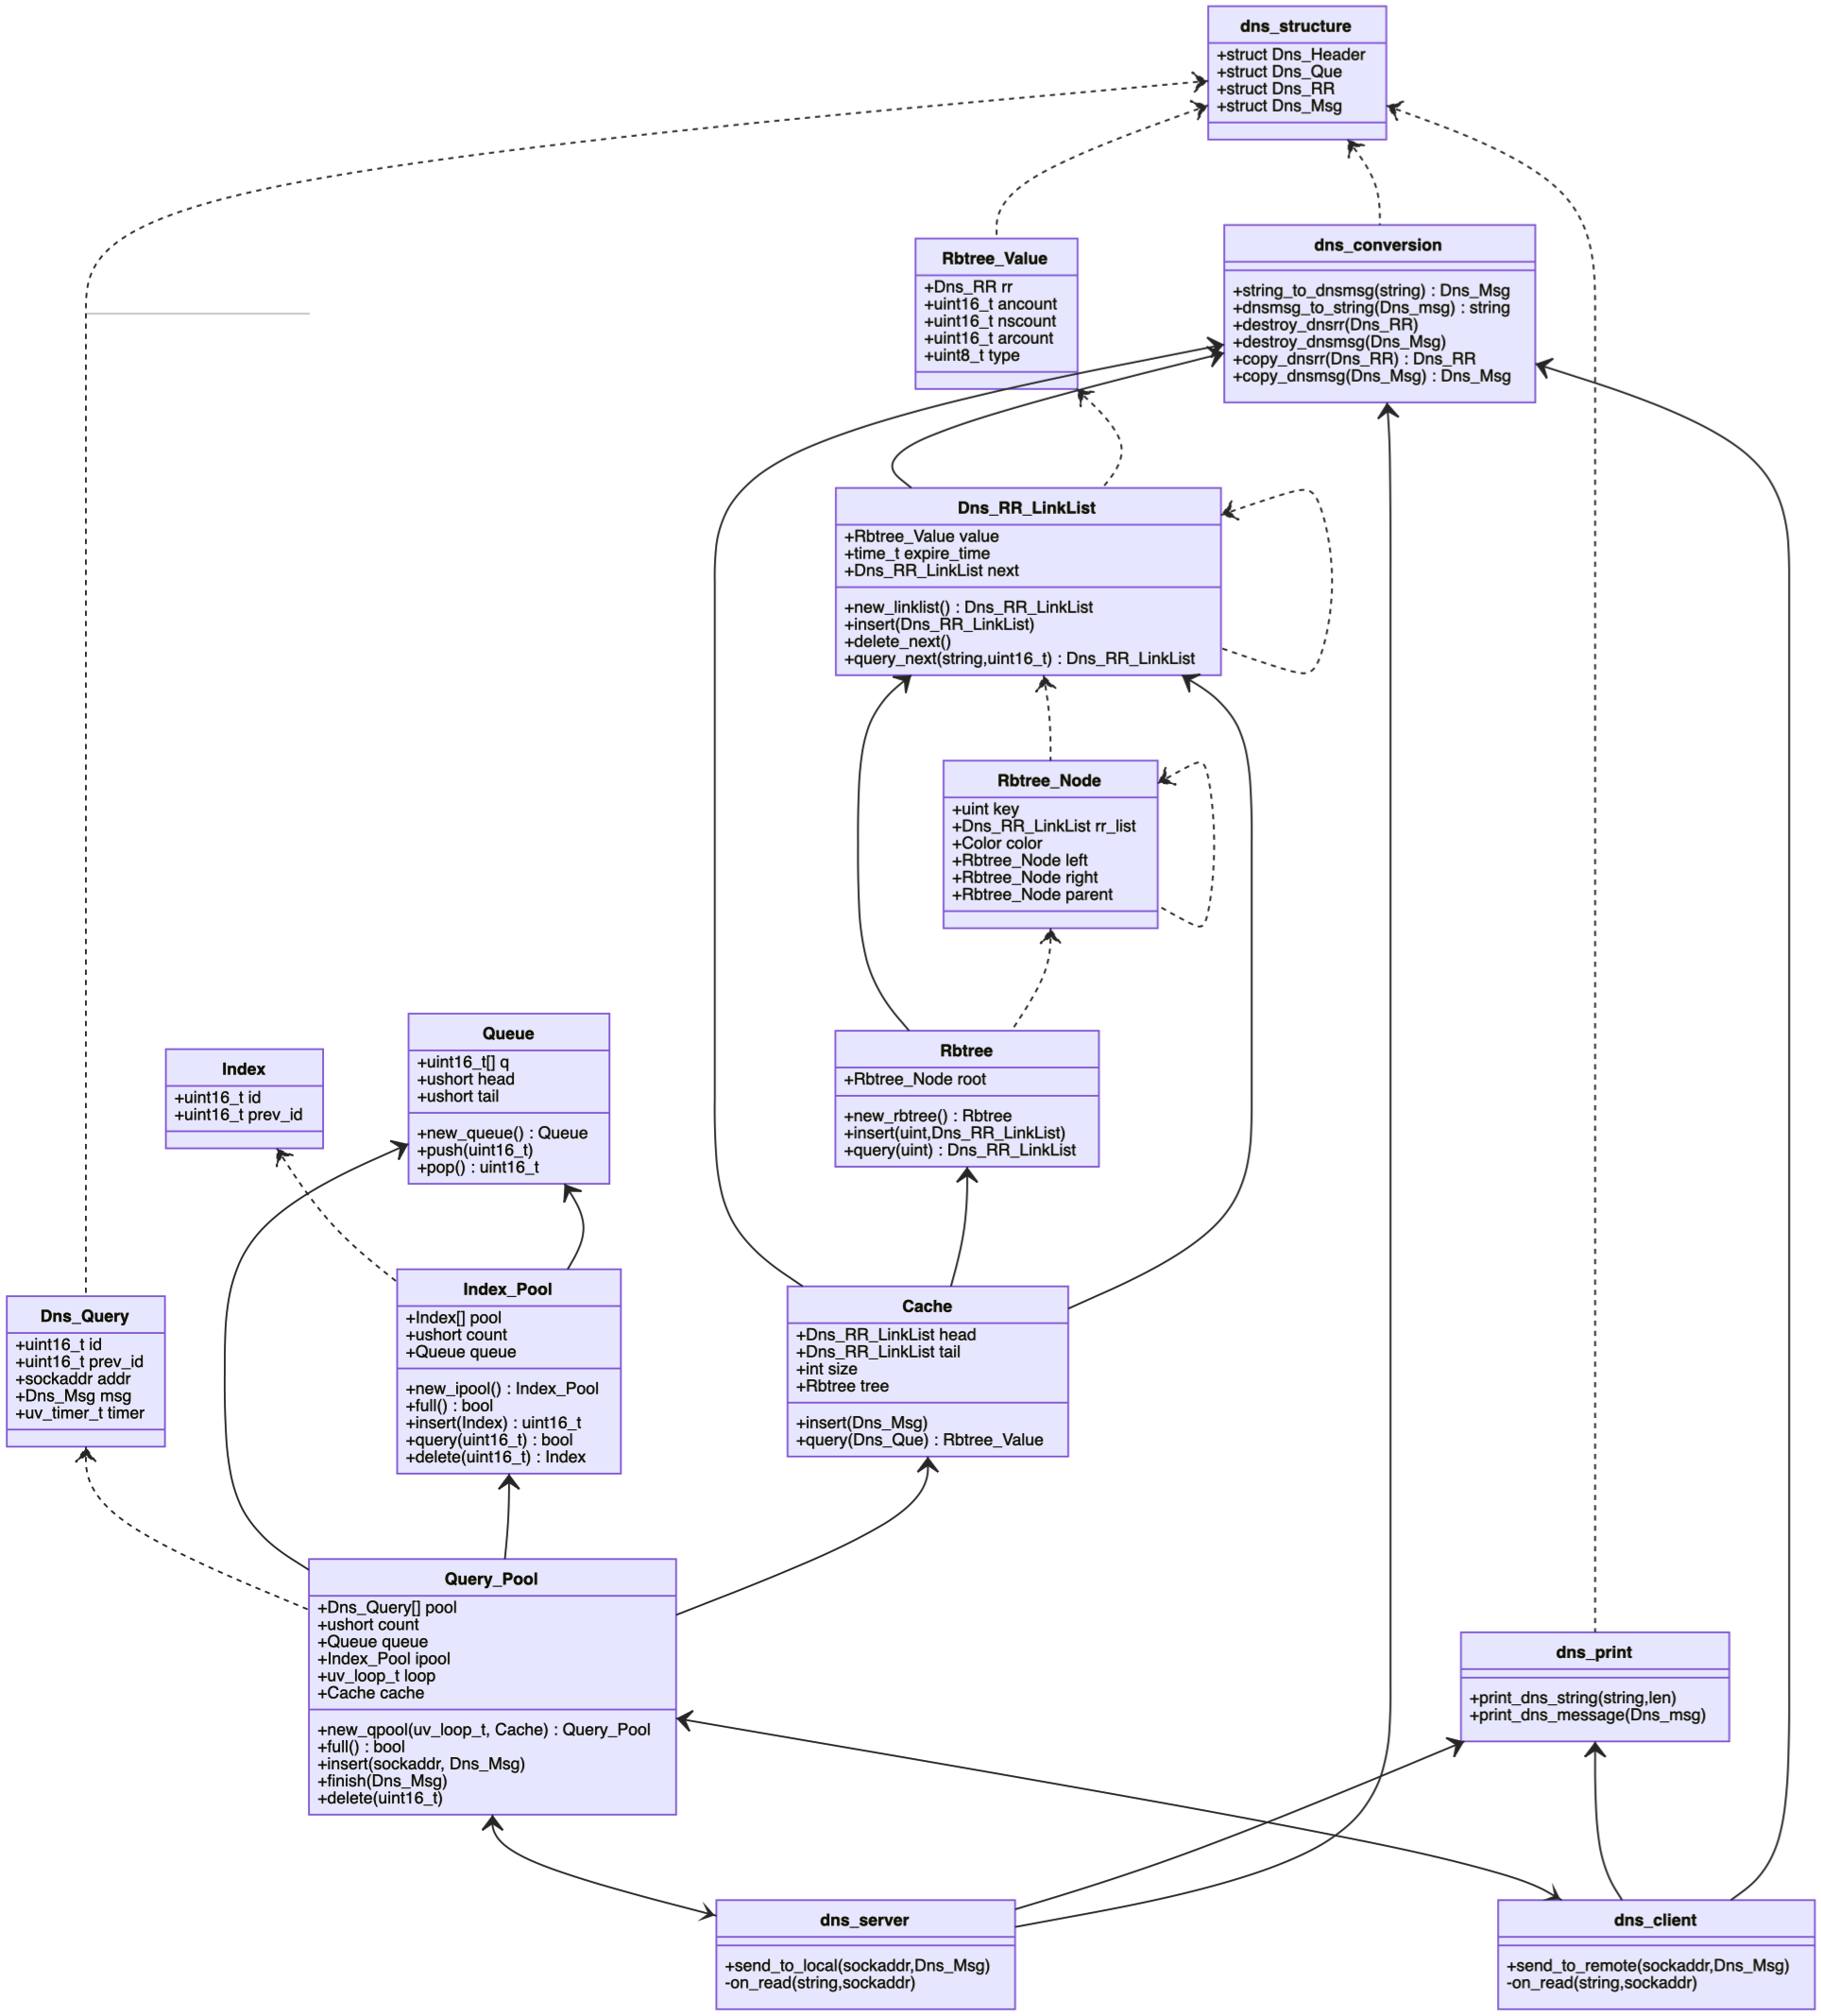
\includegraphics[width=\linewidth]{./Images/structure.png}
    \caption{模块关系图\label{fig:structure}}

\end{figure}

DNS中继服务器的基础框架包括服务端、客户端及一个查询池,服务端通过socket与本地进程通信,客户端通过socket与远程DNS服务器通信;客户端和服务端收到报文时,将其转换成结构体的形式,发送报文时,将结构体转化成字节流;中继服务器的各个模块之间通信均采用结构体的形式,相比字节流而言比较直观。中继服务器的基础框架如\figref{fig:structure2}。

\begin{figure}[htbp]

    \centering
    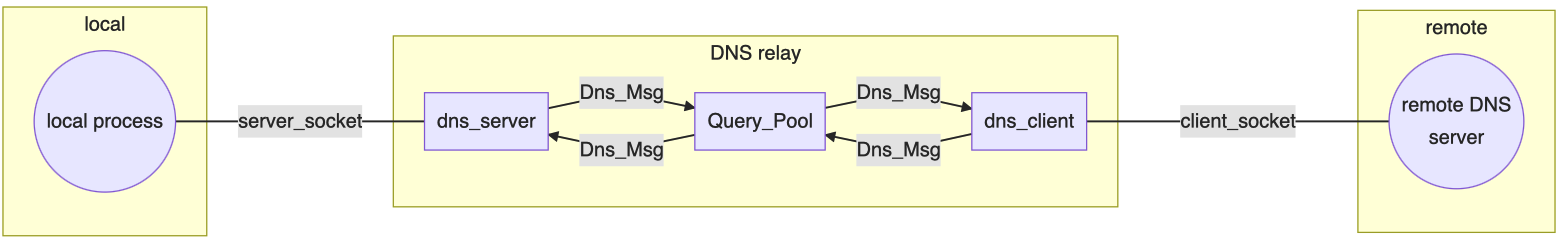
\includegraphics[width=\linewidth]{./Images/structure2.png}
    \caption{DNS中继服务器基础框架\label{fig:structure2}}

\end{figure}

此外,本地缓存分为两层,分别为一个高速缓存LRU以及一个红黑树,LRU的内容是红黑树的子集,每次查询时,首先在LRU中查找结果,再在红黑树中查找结果,如果未命中,则向远程服务器发送查询报文。当收到来自远程DNS服务器的回复报文时,会复制两个副本,分别插入到LRU和红黑树中,这三者的关系如\figref{fig:structure3}。

\begin{figure}[htbp]

    \centering
    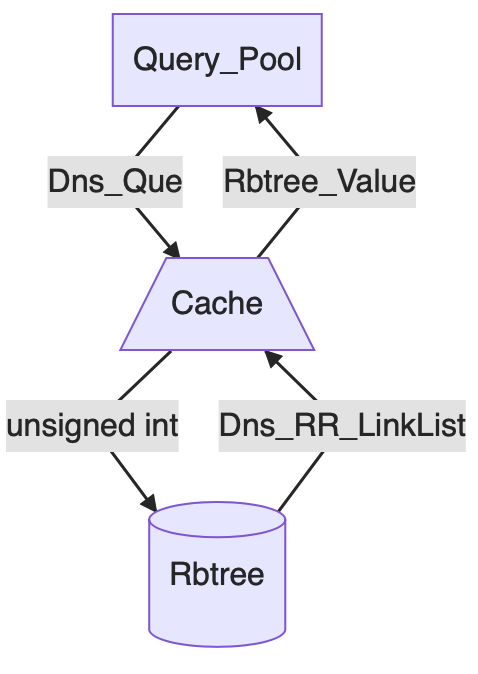
\includegraphics[width=0.3\linewidth]{./Images/structure3.png}
    \caption{查询池、高速缓存和红黑树的关系\label{fig:structure3}}

\end{figure}

\subsection{DNS报文解析和构建}

\subsubsection{DNS报文格式分析}

一个DNS报文由如下五个部分构成:

\begin{code}
\begin{minted}[frame=none]{text}
+---------------------+
|        Header       |
+---------------------+
|       Question      |
+---------------------+
|        Answer       |
+---------------------+
|      Authority      |
+---------------------+
|      Additional     |
+---------------------+
\end{minted}
\end{code}

\paragraph{Header部分格式}

Header部分为报文头,Question部分的内容为向域名服务器的查询;之后的三个部分有相同的格式,即Resource Record(RR),并且都可能为空;Answer部分是对于查询的回复,Authority部分的内容指向权威域名服务器,Additional部分包含一些相关额外信息。

Header部分的结构如下:

\begin{code}
\begin{minted}[frame=none]{text}
  0  1  2  3  4  5  6  7  8  9 10 11 12 13 14 15
+--+--+--+--+--+--+--+--+--+--+--+--+--+--+--+--+
|                      ID                       |
+--+--+--+--+--+--+--+--+--+--+--+--+--+--+--+--+
|QR|   Opcode  |AA|TC|RD|RA|   Z    |   RCODE   |
+--+--+--+--+--+--+--+--+--+--+--+--+--+--+--+--+
|                    QDCOUNT                    |
+--+--+--+--+--+--+--+--+--+--+--+--+--+--+--+--+
|                    ANCOUNT                    |
+--+--+--+--+--+--+--+--+--+--+--+--+--+--+--+--+
|                    NSCOUNT                    |
+--+--+--+--+--+--+--+--+--+--+--+--+--+--+--+--+
|                    ARCOUNT                    |
+--+--+--+--+--+--+--+--+--+--+--+--+--+--+--+--+
\end{minted}
\end{code}

\begin{itemize}
    \item ID,用于由产生DNS查询的程序分配,用于标识一个请求;一对DNS查询和回复的ID相同。
    \item QR,查询报文此位为0,回复报文此位为1。
    \item OPCODE,查询的类型:
        \begin{itemize}
            \item 0,标准查询;
            \item 1,反向查询;
            \item 2,服务器状态请求。
        \end{itemize}
    \item AA,在回复报文中有效,如果为1,表示回复Question部分查询的域名服务器是权威服务器。
    \item TC,如果为1,说明这条消息由于信道的限制而被截断。
    \item RD,在查询报文中设置,如果为1,表示期望域名服务器递归查询这个请求。
    \item RA,在回复报文中设置,如果为1,表示递归查询在域名服务器中有效。
    \item Z,预留字段,全0.
    \item RCODE,回复状态编号:
        \begin{itemize}
            \item 0,没有错误;
            \item 1,查询格式错误;
            \item 2,由于服务器错误而无法处理查询;
            \item 3,域名错误,仅在权威服务器的回复中有意义,指查询中请求的域名不存在;
            \item 4,查询的类型不受支持;
            \item 5,服务器拒绝处理请求。
        \end{itemize}
    \item QDCOUNT,Question部分中查询记录的个数(通常是1)。
    \item ANCOUNT,Answer部分中RR的个数。
    \item NSCOUNT,Authority部分中RR的个数。
    \item ARCOUNT,Additional部分中RR的个数。
\end{itemize}

\paragraph{Question部分格式}

Question部分的结构如下:

\begin{code}
\begin{minted}[frame=none]{text}
  0  1  2  3  4  5  6  7  8  9 10 11 12 13 14 15
+--+--+--+--+--+--+--+--+--+--+--+--+--+--+--+--+
|                                               |
/                     QNAME                     /
/                                               /
+--+--+--+--+--+--+--+--+--+--+--+--+--+--+--+--+
|                     QTYPE                     |
+--+--+--+--+--+--+--+--+--+--+--+--+--+--+--+--+
|                     QCLASS                    |
+--+--+--+--+--+--+--+--+--+--+--+--+--+--+--+--+
\end{minted}
\end{code}

\begin{itemize}
    \item QNAME,查询域名,格式在\ref{name_format}节说明。
    \item QTYPE,查询类型,受支持的类型如下:
        \begin{itemize}
            \item 1,A,主机地址;
            \item 2,NS,权威域名服务器;
            \item 5,CNAME,域名引用;
            \item 6,SOA,授权机构起始;
            \item 12,PTR,域名指针,用于反向域名查找;
            \item 13,HINFO,主机信息;
            \item 14,MINFO,邮箱或邮件列表信息;
            \item 15,MX,邮件交换;
            \item 16,TXT,字符串。
            \item 28,AAAA,IPv6地址。
        \end{itemize}
    \item QCLASS,查询类别,仅支持1,IN,因特网。
\end{itemize}

\paragraph{Resource Record格式}

Resource Record的格式如下:

\begin{code}
\begin{minted}[frame=none]{text}
  0  1  2  3  4  5  6  7  8  9 10 11 12 13 14 15
+--+--+--+--+--+--+--+--+--+--+--+--+--+--+--+--+
|                                               |
/                      NAME                     /
/                                               /
+--+--+--+--+--+--+--+--+--+--+--+--+--+--+--+--+
|                      TYPE                     |
+--+--+--+--+--+--+--+--+--+--+--+--+--+--+--+--+
|                     CLASS                     |
+--+--+--+--+--+--+--+--+--+--+--+--+--+--+--+--+
|                      TTL                      |
|                                               |
+--+--+--+--+--+--+--+--+--+--+--+--+--+--+--+--+
|                    RDLENGTH                   |
+--+--+--+--+--+--+--+--+--+--+--+--+--+--+--+--+
|                                               |
/                     RDATA                     /
/                                               /
+--+--+--+--+--+--+--+--+--+--+--+--+--+--+--+--+
\end{minted}
\end{code}

\begin{itemize}
    \item NAME,此RR从属的域名,格式在\ref{name_format}节说明。
    \item TYPE,RR类型,支持的类型与QTYPE部分相同。
    \item CLASS,RR类别,仅支持1,IN,因特网。
    \item TTL,期望此RR被缓存的时间。
    \item RDLENGTH,RDATA部分的长度。
    \item RDATA,资源内容,根据TYPE的不同,其内容也不同。
\end{itemize}

\paragraph{域名格式}
\label{name_format}

Question部分和RR中的域名都是由一串字符\mintinline{text}{<domain-name>}表示,一般由0表示终止,其长度任意,并且不包含填充。
\mintinline{text}{<domain-name>}由若干个\mintinline{text}{<character-string>}构成,每个\mintinline{text}{<character-string>}由一个八位数字开头,之后跟着长度等于这个数字的字符串。\mintinline{text}{<character-string>}最多包含256个字符。

为了压缩DNS报文的长度,增大传输效率,引入了域名的压缩,此时\mintinline{text}{<domain-name>}可能由0或者一个指针终止,一个指针由两个字节构成,其格式如下:

\begin{code}
\begin{minted}[frame=none]{text}
+--+--+--+--+--+--+--+--+--+--+--+--+--+--+--+--+
| 1  1|                OFFSET                   |
+--+--+--+--+--+--+--+--+--+--+--+--+--+--+--+--+
\end{minted}
\end{code}

这个指针指向从DNS报文头起第\mintinline{text}{OFFSET}个字节,原本域名的剩余部分应该从这个字节开始继续读取。

\paragraph{RDATA格式}

对于DNS中继服务器来说,RDATA部分的内容并不重要,只是涉及到域名压缩,以及调试输出的需求,所以需要对一部分类型的RDATA作处理。需要处理的RDATA如下。

\subparagraph{A类型RDATA格式}

如下:

\begin{code}
\begin{minted}[frame=none]{text}
    +--+--+--+--+--+--+--+--+--+--+--+--+--+--+--+--+
    |                    ADDRESS                    |
    +--+--+--+--+--+--+--+--+--+--+--+--+--+--+--+--+
\end{minted}
\end{code}

\begin{itemize}
    \item ADDRESS,32位IPv4地址。
\end{itemize}

\subparagraph{NS/CNAME类型RDATA格式}

如下:

\begin{code}
\begin{minted}[frame=none]{text}
    +--+--+--+--+--+--+--+--+--+--+--+--+--+--+--+--+
    |                     NAME                      |
    +--+--+--+--+--+--+--+--+--+--+--+--+--+--+--+--+
\end{minted}
\end{code}

\begin{itemize}
    \item NAME,一个域名。
\end{itemize}

\subparagraph{MX类型RDATA格式}

如下:

\begin{code}
\begin{minted}[frame=none]{text}
    +--+--+--+--+--+--+--+--+--+--+--+--+--+--+--+--+
    |                  PREFERENCE                   |
    +--+--+--+--+--+--+--+--+--+--+--+--+--+--+--+--+
    |                   EXCHANGE                    |
    +--+--+--+--+--+--+--+--+--+--+--+--+--+--+--+--+
\end{minted}
\end{code}

\begin{itemize}
    \item PREFERENCE,16位数字。
    \item EXCHANGE,一个域名。
\end{itemize}

\subparagraph{SOA类型RDATA格式}

如下:

\begin{code}
\begin{minted}[frame=none]{text}
    +--+--+--+--+--+--+--+--+--+--+--+--+--+--+--+--+
    |                                               |
    /                     MNAME                     /
    /                                               /
    +--+--+--+--+--+--+--+--+--+--+--+--+--+--+--+--+
    |                                               |
    /                     RNAME                     /
    /                                               /
    +--+--+--+--+--+--+--+--+--+--+--+--+--+--+--+--+
    |                    SERIAL                     |
    |                                               |
    +--+--+--+--+--+--+--+--+--+--+--+--+--+--+--+--+
    |                    REFRESH                    |
    |                                               |
    +--+--+--+--+--+--+--+--+--+--+--+--+--+--+--+--+
    |                     RETRY                     |
    |                                               |
    +--+--+--+--+--+--+--+--+--+--+--+--+--+--+--+--+
    |                    EXPIRE                     |
    |                                               |
    +--+--+--+--+--+--+--+--+--+--+--+--+--+--+--+--+
    |                    MINIMUM                    |
    |                                               |
    +--+--+--+--+--+--+--+--+--+--+--+--+--+--+--+--+
\end{minted}
\end{code}

\begin{itemize}
    \item MNAME,一个域名。
    \item RNAME,一个域名。
    \item SERIAL,一个32位数字。
    \item REFRESH,一个32位数字。
    \item RETRY,一个32位数字。
    \item EXPIRE,一个32位数字。
    \item MINIMUM,一个32位数字。
\end{itemize}

\subparagraph{AAAA类型RDATA格式}

如下:

\begin{code}
\begin{minted}[frame=none]{text}
    +--+--+--+--+--+--+--+--+--+--+--+--+--+--+--+--+
    |                                               |
    |                                               |
    |                                               |
    |                    ADDRESS                    |
    |                                               |
    |                                               |
    |                                               |
    |                                               |
    +--+--+--+--+--+--+--+--+--+--+--+--+--+--+--+--+
\end{minted}
\end{code}

\begin{itemize}
    \item ADDRESS,128位IPv6地址。
\end{itemize}

\subsubsection{DNS报文结构体}

DNS报文结构体定义在\mintinline{text}{dns_structure.h}中,由四个结构体构成,其结构如\figref{fig:struct_structure}所示。

\begin{figure}[htbp]

    \centering
    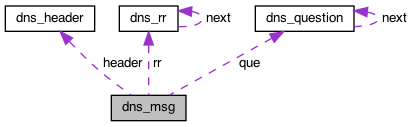
\includegraphics[width=0.7\linewidth]{./APIdoc/structdns__msg__coll__graph.png}
    \caption{DNS报文结构体的结构\label{fig:struct_structure}}

\end{figure}

Header部分长度固定,其中部分不足一个字节的字段采用位域(bit field)的方式定义,节省空间;
Question部分的查询记录个数不定,采用单向链表实现,便于顺序访问;之后的Answer、Authority和Additional部分的格式相同,采用一个单向链表顺序连接起来。

四个结构体的定义如下所示:

\begin{code}
\begin{minted}{C}
typedef struct dns_header
{
    uint16_t id;
    uint8_t qr: 1;
    uint8_t opcode: 4;
    uint8_t aa: 1;
    uint8_t tc: 1;
    uint8_t rd: 1;
    uint8_t ra: 1;
    uint8_t z: 3;
    uint8_t rcode: 4;
    uint16_t qdcount;
    uint16_t ancount;
    uint16_t nscount;
    uint16_t arcount;
} Dns_Header;
 
typedef struct dns_question
{
    uint8_t * qname;
    uint16_t qtype;
    uint16_t qclass;
    struct dns_question * next;
} Dns_Que;
 
typedef struct dns_rr
{
    uint8_t * name;
    uint16_t type;
    uint16_t class;
    uint32_t ttl;
    uint16_t rdlength;
    uint8_t * rdata;
    struct dns_rr * next;
} Dns_RR;
 
typedef struct dns_msg
{
    Dns_Header * header; 
    Dns_Que * que; 
    Dns_RR * rr; 
} Dns_Msg;
\end{minted}
\end{code}

\mintinline{text}{dns_structure.h}的文档见\href{run:./APIdoc/dns__structure_8h.html}{dns\_structure.h文件参考}。

\subsubsection{DNS报文字节流和结构体的转换}

从UDP socket中获取到的DNS报文是字节流的形式,我们需要将它转换成结构体,便于分析与输出,之后需要将结构体转换回字节流进行发送。

此外,我们还需要关注报文结构体和RR结构体的复制和销毁操作。

上述操作定义在\mintinline{text}{dns_conversion.h}中,如下:

\begin{code}
\begin{minted}{C}
void string_to_dnsmsg(Dns_Msg * pmsg, const char * pstring);

unsigned dnsmsg_to_string(const Dns_Msg * pmsg, char * pstring);
 
void destroy_dnsrr(Dns_RR * prr);
 
void destroy_dnsmsg(Dns_Msg * pmsg);
 
Dns_RR * copy_dnsrr(const Dns_RR * src);
 
Dns_Msg * copy_dnsmsg(const Dns_Msg * src);
\end{minted}
\end{code}

\mintinline{text}{dns_conversion.h}的文档见\href{run:./APIdoc/dns__conversion_8h.html}{dns\_conversion.h文件参考}。

\paragraph{将字节流转换成结构体}

\mintinline{C}{string_to_dnsmsg}函数实现将字节流转换成结构体,它的函数调用图如\figref{fig:string_to_dnsmsg_call}。

\begin{figure}[htbp]

    \centering
    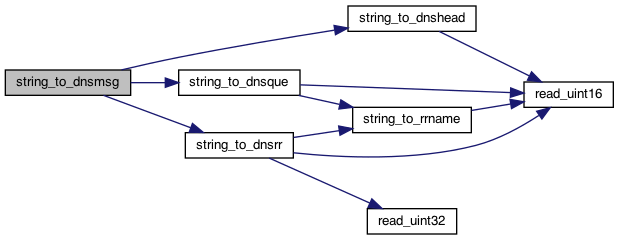
\includegraphics[width=0.8\linewidth]{./APIdoc/dns__conversion_8c_a0f89102e256c499ffa19784791cb68f6_cgraph.png}
    \caption{\mintinline{C}{string_to_dnsmsg}函数调用图\label{fig:string_to_dnsmsg_call}}

\end{figure}

从图中可见,此函数分别调用\mintinline{C}{string_to_dnshead}、\mintinline{C}{string_to_dnsque}和\mintinline{C}{string_to_dnsrr}将报文的三个部分转换为结构体,对于Question部分和RR部分,需要维护一个链表头指针和尾指针,每次转换后的新记录插入链表尾即可。

此外,考虑到域名格式的特殊性,\mintinline{C}{string_to_rrname}函数负责通过递归的形式将域名解析成可输出的常见的格式,\mintinline{C}{read_uint16}和\mintinline{C}{read_uint32}函数用于将大端法数字转换成小端法数字。

\paragraph{将结构体转换成字节流}

\mintinline{C}{dnsmsg_to_string}函数实现将结构体转换成字节流,它的函数调用图如\figref{fig:dnsmsg_to_string_call}。

\begin{figure}[htbp]

    \centering
    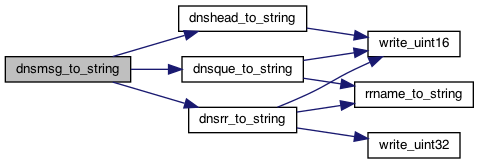
\includegraphics[width=0.7\linewidth]{./APIdoc/dns__conversion_8c_aa893e182a92c2ccf5644c1f8a12fba37_cgraph.png}
    \caption{\mintinline{C}{dnsmsg_to_string}函数调用图\label{fig:dnsmsg_to_string_call}}

\end{figure}

\mintinline{C}{dnsmsg_to_string}函数基本上是\mintinline{C}{string_to_dnsmsg}的逆过程,分别调用类似的六个函数实现相应的功能。

\paragraph{结构体的销毁}

\mintinline{C}{destroy_dnsmsg}和\mintinline{C}{destroy_dnsrr}函数分别实现整个DNS报文的销毁和RR链表的销毁。

\paragraph{结构体的复制}

\mintinline{C}{copy_dnsmsg}和\mintinline{C}{copy_dnsrr}函数分别实现整个DNS报文的复制和RR链表的复制。

上面提到的函数接口的的文档见\href{run:./APIdoc/dns__conversion_8c.html}{dns\_conversion.c文件参考}。

\subsubsection{DNS报文的输出}

通过输出DNS字节流和结构体,可以观察DNS报文的转换过程是否正确,并且跟踪程序运行的过程,便于debug的工作。

上述操作定义在\mintinline{text}{dns_print.h}中,如下:

\begin{code}
\begin{minted}{C}
void print_dns_string(const char * pstring, unsigned int len);
 
void print_dns_message(const Dns_Msg * pmsg);
\end{minted}
\end{code}

\mintinline{text}{dns_print.h}的文档见\href{run:./APIdoc/dns__print_8h.html}{dns\_print.h文件参考}。

\mintinline{C}{print_dns_string}函数用于输出DNS字节流,输出的效果如下:

\begin{code}
\begin{minted}[frame=none]{text}
0000 bd da 81 80 00 01 00 01 00 00 00 00 03 77 77 77 
0010 04 62 75 70 74 03 65 64 75 02 63 6e 00 00 01 00 
0020 01 03 77 77 77 04 62 75 70 74 03 65 64 75 02 63 
0030 6e 00 00 01 00 01 ff ff ff ff 00 04 0a 03 09 a1 
\end{minted}
\end{code}

\mintinline{C}{print_dns_message}函数用于输出DNS结构体,其函数调用图如\figref{fig:print_dns_message_call}。

\begin{figure}[htbp]

    \centering
    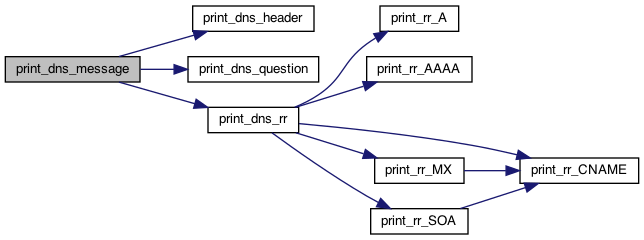
\includegraphics[width=0.8\linewidth]{./APIdoc/dns__print_8c_a33a39397e0f2e1a98b86b6d85321ee79_cgraph.png}
    \caption{\mintinline{C}{print_dns_message}函数调用图\label{fig:print_dns_message_call}}

\end{figure}

该函数分别调用\mintinline{C}{print_dns_header}、\mintinline{C}{print_dns_question}和\mintinline{C}{print_dns_rr}函数输出结构体的三个部分。
由于RR的RDATA字段格式较多,所以另外实现了几个函数分别用于输出A、AAAA、MX(NS)、CNAME、SOA类型的RDATA字段。

输出的效果如下:

\begin{code}
\begin{minted}[frame=none]{text}
=======Header==========
ID = 0xbdda
QR = 1
OPCODE = 0
AA = 0
TC = 0
RD = 1
RA = 1
RCODE = 0
QDCOUNT = 1
ANCOUNT = 1
NSCOUNT = 0
ARCOUNT = 0

=======Question========
QNAME = www.bupt.edu.cn.
QTYPE = 1
QCLASS = 1

=======Answer==========
NAME = www.bupt.edu.cn.
TYPE = 1
CLASS = 1
TTL = 4294967295
RDLENGTH = 4
RDATA = 10.3.9.161

=======Authority=======
=======Additional======
\end{minted}
\end{code}

上面提到的函数接口的的文档见\href{run:./APIdoc/dns__print_8c.html}{dns\_print.c文件参考}。

\subsection{DNS记录的存储}

理论上,通过一个域名和类型可以查询到一个RR的列表作为回复。对于DNS记录的存储就是基于这个对应关系。

\subsubsection{红黑树和RR链表}

DNS记录存储在一个红黑树中,红黑树节点的键是域名字符串经过哈希得到的整数,由于哈希可能存在冲突,并且一个域名可能对应多个不同类的查询,可采用拉链法解决冲突。
因此,每个红黑树节点对应多个值,这些值被串联成一个有空头结点的单向链表。每个值中存储域名和查询类型、一个RR的列表和RR列表中各个部分的个数。

上述数据结构的结构体的关系如\figref{fig:rbtree_structure}所示。

\begin{figure}[htbp]

    \centering
    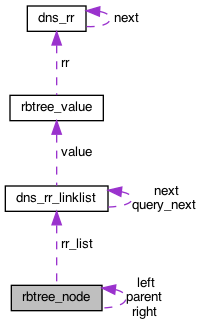
\includegraphics[width=0.3\linewidth]{./APIdoc/structrbtree__node__coll__graph.png}
    \caption{红黑树和RR链表结构体的关系\label{fig:rbtree_structure}}

\end{figure}

红黑树中会存储从对照表中读取到的”IP地址-域名“对,也会存储运行时收到的回复。当存储对照表中的记录时,默认这些记录是永久的,而存储运行时的回复时,需要根据RR列表中最小的TTL确认这条记录的过期时间,过期时间记录在链表的节点中。

此外,红黑树和RR链表(以及之后的大部分数据结构)都将数据结构的操作作为函数指针封装在结构体中,达到类似成员函数的效果。

红黑树和RR链表的数据结构和操作定义在\mintinline{text}{rbtree.h}中,如下:

\begin{code}
\begin{minted}{C}
typedef enum
{
    BLACK, RED
} Color;
 
typedef struct rbtree_value
{
    Dns_RR * rr; 
    uint16_t ancount; 
    uint16_t nscount; 
    uint16_t arcount; 
    uint8_t type; 
} Rbtree_Value;
 
typedef struct dns_rr_linklist
{
    Rbtree_Value * value; 
    time_t expire_time; 
    struct dns_rr_linklist * next; 
    
    void (* insert)(struct dns_rr_linklist * list, struct dns_rr_linklist * new_list_node);
    
    void (* delete_next)(struct dns_rr_linklist * list);
    
    struct dns_rr_linklist * (* query_next)(struct dns_rr_linklist * list, const uint8_t * qname, const uint16_t qtype);
} Dns_RR_LinkList;
 
typedef struct rbtree_node
{
    unsigned int key; 
    Dns_RR_LinkList * rr_list; 
    Color color; 
    struct rbtree_node * left; 
    struct rbtree_node * right; 
    struct rbtree_node * parent; 
} Rbtree_Node;
 
typedef struct rbtree
{
    Rbtree_Node * root; 
    
    void (* insert)(struct rbtree * tree, unsigned int key, Dns_RR_LinkList * list);
    
    Dns_RR_LinkList * (* query)(struct rbtree * tree, unsigned int data);
} Rbtree;
 
Dns_RR_LinkList * new_linklist();
 
Rbtree * new_rbtree();
\end{minted}
\end{code}

\mintinline{text}{rbtree.h}的文档见\href{run:./APIdoc/rbtree_8h.html}{rbtree.h文件参考}。

\paragraph{RR链表}\label{rr_linklist}

\mintinline{C}{Dns_RR_LinkList}结构体有三个方法:

\begin{itemize}
    \item \mintinline{C}{insert}方法用于在链表中的某个节点后插入新节点。
    \item \mintinline{C}{delete_next}方法用于删除链表中某个节点的下一个结点。
    \item \mintinline{C}{query_next}方法用于遍历一个链表,根据域名和查询类型从中筛选出一个节点。
\end{itemize}

此外,\mintinline{C}{new_linklist}函数用于创建一个新的RR链表节点。

\paragraph{红黑树的插入操作}

\mintinline{C}{Rbtree}结构体的\mintinline{C}{insert}方法用于向红黑树中插入键-值对。

具体来说,函数传入一个键和一个RR链表节点。首先在红黑树中按照键查找对应的节点,如果查找到节点,则将RR链表节点插入这个节点的RR链表尾;如果查找不到节点,则创建一个新节点以及一个有空头结点的RR链表,并将传入的RR链表节点插入到这个链表尾,在此之后,需要调用\mintinline{C}{insert_case}函数维护红黑树的平衡。

对于红黑树的维护细节不属于本报告的范畴,故略去。

这个方法对应\mintinline{text}{rbtree.c}中的\mintinline{C}{rbtree_insert}函数,该函数的调用图如\figref{fig:rbtree_insert_call}所示。

\begin{figure}[htbp]

    \centering
    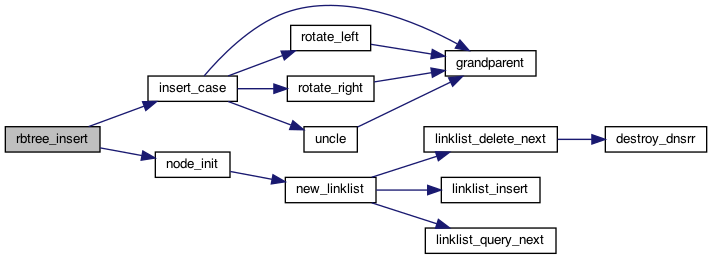
\includegraphics[width=0.8\linewidth]{./APIdoc/rbtree_8c_ae46c23eec5c1ea21ebab9279843de3a3_cgraph.png}
    \caption{\mintinline{C}{rbtree_insert}函数的调用图\label{fig:rbtree_insert_call}}

\end{figure}

\paragraph{红黑树的查询操作}

\mintinline{C}{Rbtree}结构体的\mintinline{C}{query}方法用于根据键在红黑树中查询RR链表。

函数调用\mintinline{C}{rbtree_find}函数,在红黑树中根据键查找结点。如果查找到节点,将节点的RR链表中超时的节点删去。如果此时节点的链表为空(即只有一个头节点),则调用\mintinline{C}{rbtree_delete}函数删除这个节点,并且维护红黑树的平衡;否则返回这个RR链表。

这个方法对应\mintinline{text}{rbtree.c}中的\mintinline{C}{rbtree_query}函数,该函数的调用图如\figref{fig:rbtree_query_call}所示。

\begin{figure}[htbp]

    \centering
    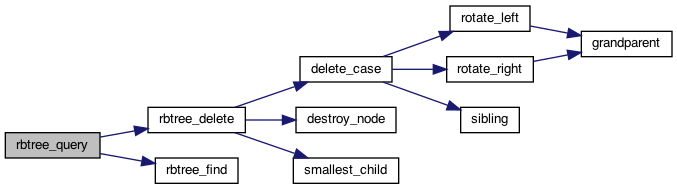
\includegraphics[width=0.8\linewidth]{./APIdoc/rbtree_8c_a7460cf092b0132ece0a692cd84a26456_cgraph.png}
    \caption{\mintinline{C}{rbtree_query}函数的调用图\label{fig:rbtree_query_call}}

\end{figure}

此外,\mintinline{C}{new_rbtree}函数用于创建一棵新的空红黑树。

上面提到的函数接口的的文档见\href{run:./APIdoc/rbtree_8c.html}{rbtree.c文件参考}。

\subsubsection{LRU高速缓存}

对于经常访问的缓存,将其存储到高速缓存中可以加快查询速度。利用\ref{rr_linklist}节提到的RR链表,我们实现了一个LRU(Least Recently Used,最近最少使用)缓存。

对于在这个RR链表中,最近被访问的记录会被移到链表尾,当链表长度达到上限时,优先移出链表头的节点,即最久未使用的值最先被移出缓存。

缓存的数据结构和操作定义在\mintinline{text}{cache.h}中,如下:

\begin{code}
\begin{minted}{C}
#define CACHE_SIZE 30
 
typedef struct cache_
{
    Dns_RR_LinkList * head; 
    Dns_RR_LinkList * tail; 
    int size; 
    Rbtree * tree; 
    
    void (* insert)(struct cache_ * cache, const Dns_Msg * msg);
    
    Rbtree_Value * (* query)(struct cache_ * cache, const Dns_Que * que);
} Cache;
 
Cache * new_cache(FILE * hosts_file);
\end{minted}
\end{code}

\mintinline{text}{cache.h}的文档见\href{run:./APIdoc/cache_8h.html}{cache.h文件参考}。

\paragraph{缓存的初始化}

\mintinline{C}{new_cache}函数用于创建一个新的缓存。

此函数会调用\mintinline{C}{new_rbtree}创建一棵新的红黑树,之后从对照表的文件中读入“域名-IP”对,构造RR记录和RR链表节点并插入红黑树中。

一个对照表的例子如下:

\label{iptable}
\begin{code}
\begin{minted}{text}
baidu.com 220.181.38.148
www.cloudflare.com 104.16.124.96
www.bupt.edu.cn 10.3.9.161
google.com 172.217.160.78
test.com 0.0.0.0
bt.byr.cn 2001:da8:215:4078:250:56ff:fe97:654d
\end{minted}
\end{code}

\paragraph{缓存的插入操作} 

\mintinline{C}{Cache}结构体的\mintinline{C}{insert}方法用于向缓存中插入DNS记录。

该函数会从DNS报文数据结构中提取出QNAME、QTYPE、ANCOUNT、NSCOUNT、ARCOUNT,将RR部分复制两遍以创建两个RR链表节点,将这两个节点分别插入LRU缓存中和红黑树中。

函数调用\mintinline{C}{BKDRHash}函数对域名生成字符串哈希,调用\mintinline{C}{get_min_ttl}得到一个RR列表中最小的TTL。

这个方法对应\mintinline{text}{cache.c}中的\mintinline{C}{cache_insert}函数,该函数的调用图如\figref{fig:cache_insert_call}所示。

\begin{figure}[htbp]

    \centering
    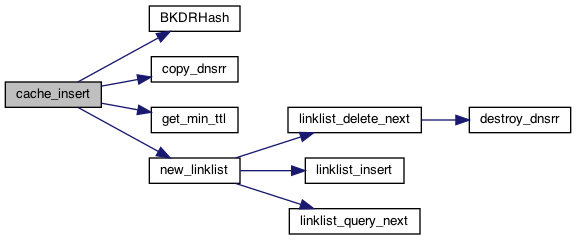
\includegraphics[width=0.8\linewidth]{./APIdoc/cache_8c_a6ced4e1f620d2e750fb0c2c049962fa8_cgraph.png}
    \caption{\mintinline{C}{cache_insert}函数的调用图\label{fig:cache_insert_call}}

\end{figure}

\paragraph{缓存的查询操作}

\mintinline{C}{Cache}结构体的\mintinline{C}{query}方法用于在缓存中查询DNS记录。

该函数会首先在LRU中查询DNS记录,如果查询到,将该节点移到链表的末尾,之后生成该节点中的值的副本并且返回;

如果在LRU中查找不到,则调用红黑树的\mintinline{C}{query}方法进行查询,在返回的链表中查找满足QNAME和QTYPE的值,将查找到的值复制两份,一份插入到LRU缓存中,一份返回。

如果红黑树中也查找不到,则返回空指针。

这个方法对应\mintinline{text}{cache.c}中的\mintinline{C}{cache_query}函数,该函数的调用图如\figref{fig:cache_query_call}所示。

\begin{figure}[htbp]

    \centering
    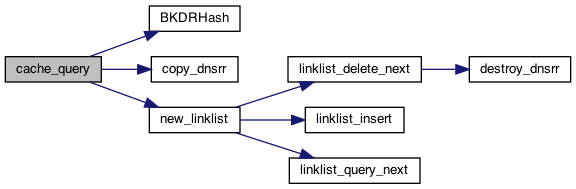
\includegraphics[width=0.8\linewidth]{./APIdoc/cache_8c_a1abbd81313d8d7e8b25446d7921121e0_cgraph.png}
    \caption{\mintinline{C}{cache_query}函数的调用图\label{fig:cache_query_call}}

\end{figure}

上面提到的函数接口的的文档见\href{run:./APIdoc/cache_8c.html}{cache.c文件参考}。

\subsection{序号池和查询池}

为了实现并发查询,我们实现了一个查询池,查询池中的内容为DNS查询。中继服务器会为每个DNS查询分配一个序号,同时保存以下信息:

\begin{itemize}
    \item 请求方的地址,中继服务器向这个地址发送回复。
    \item 原本的DNS查询报文,中继服务器收到远程回复时和原本的查询报文比对。
    \item 计时器,DNS查询超时后自动从查询池中移除并销毁。
\end{itemize}

为了防止短时间内查询序号重复,导致无法区分当前查询和之前的查询,我们采用滑动窗口的方式分配查询序号。查询池的大小为256,而查询序号为0至65535。

具体来说,查询池外维护一个队列,队列中保存未使用的查询序号,初始情况下,队列中有0至255的序号;当需要在查询池中添加查询时,从队列中取出一个序号并创建新的DNS查询;当一个从查询池中移除一个查询时,将它的查询编号加256后再加入队列。

DNS报文中的ID是由不同进程自主生成的,为了区分不同的报文,中继服务器在向远程服务器发送报文之前,需要重新分配报文ID,并且建立报文ID和DNS查询序号的对应关系。

因此,我们另外实现了一个序号池,实现方式和查询池类似,即采用一个队列保存未分配的序号,需要分配新序号时从队列里取出并加入查询池,序号用完后从查询池中移除并加入队列。在分配序号时不需要考虑重复的情况,所以序号池的大小为65536。

\subsubsection{队列}

为了节省空间,我们实现了一个循环队列,大小为65536。队列的下标采用自然溢出的方式。

队列的数据结构和操作定义在\mintinline{text}{queue.h}中,如下:

\begin{code}
\begin{minted}{C}
#define QUEUE_MAX_SIZE 65536

typedef struct queue
{
    uint16_t q[QUEUE_MAX_SIZE]; 
    unsigned short head; 
    unsigned short tail; 
    
    void (* push)(struct queue * queue, uint16_t num);
    
    uint16_t (* pop)(struct queue * queue);
    
    void (* destroy)(struct queue * queue);
} Queue;
 
Queue * new_queue();
\end{minted}
\end{code}

\mintinline{text}{queue.h}的文档见\href{run:./APIdoc/queue_8h.html}{queue.h文件参考}。

\paragraph{队列的初始化}

\mintinline{C}{new_queue}函数用于创建一个新的队列。

\paragraph{队列的入队操作}

\mintinline{C}{Queue}结构体的\mintinline{C}{push}方法用于向队尾插入值。

\paragraph{队列的出队操作}

\mintinline{C}{Queue}结构体的\mintinline{C}{pop}方法取出队首的值并返回。

\paragraph{队列的销毁}

\mintinline{C}{Queue}结构体的\mintinline{C}{destroy}方法销毁队列。

上面提到的函数接口的的文档见\href{run:./APIdoc/queue_8c.html}{queue.c文件参考}。

\subsubsection{序号池}

如前所述,我们定义一个结构体保存报文的序号及其对应查询的序号。一个报文序号在序号池中的位置是固定的(即,如果结构体中的序号是x,则查询池中下标为x的指针指向这个结构体),所以判断一个序号是否在序号池中,只需要判断序号池中对应位置的指针是否为空即可。

序号池的数据结构和操作定义在\mintinline{text}{index_pool.h}中,如下:

\begin{code}
\begin{minted}{C}
#define INDEX_POOL_MAX_SIZE 65535

typedef struct index_
{
    uint16_t id; 
    uint16_t prev_id; 
} Index;
 
typedef struct index_pool
{
    Index * pool[INDEX_POOL_MAX_SIZE]; 
    unsigned short count; 
    Queue * queue; 
    
    bool (* full)(struct index_pool * ipool);
    
    uint16_t (* insert)(struct index_pool * ipool, Index * req);
    
    bool (* query)(struct index_pool * ipool, uint16_t index);
    
    Index * (* delete)(struct index_pool * ipool, uint16_t index);
    
    void (* destroy)(struct index_pool * ipool);
} Index_Pool;
 
Index_Pool * new_ipool();
\end{minted}
\end{code}

\mintinline{text}{index_pool.h}的文档见\href{run:./APIdoc/index__pool_8h.html}{index\_pool.h文件参考}。

\paragraph{序号池的初始化}

\mintinline{C}{new_ipool}函数用于创建一个新的序号池。

\paragraph{判断序号池满}

\mintinline{C}{Index_Pool}结构体的\mintinline{C}{full}方法用于判断序号池是否已满。

\paragraph{序号池的插入操作}

\mintinline{C}{Index_Pool}结构体的\mintinline{C}{insert}方法从队首取出序号加入序号池。

\paragraph{序号池的移除操作}

\mintinline{C}{Index_Pool}结构体的\mintinline{C}{delete}方法从序号池中删除给定的序号,并且将序号插入队列。

\paragraph{序号池的销毁}

\mintinline{C}{Index_Pool}结构体的\mintinline{C}{destroy}方法销毁序号池。

上面提到的函数接口的的文档见\href{run:./APIdoc/index__pool_8c.html}{index\_pool.c文件参考}。

\subsubsection{查询池}

如前所述,我们定义一个结构体表示DNS查询,以及另一个结构体表示查询池。

查询池的数据结构和操作定义在\mintinline{text}{query_pool.h}中,如下:

\begin{code}
\begin{minted}{C}
#define QUERY_POOL_MAX_SIZE 256

typedef struct dns_query
{
    uint16_t id; 
    uint16_t prev_id; 
    struct sockaddr addr; 
    Dns_Msg * msg; 
    uv_timer_t timer; 
} Dns_Query;
 
typedef struct query_pool
{
    Dns_Query * pool[QUERY_POOL_MAX_SIZE]; 
    unsigned short count; 
    Queue * queue; 
    Index_Pool * ipool; 
    uv_loop_t * loop; 
    Cache * cache; 
    
    bool (* full)(struct query_pool * qpool);
    
    void (* insert)(struct query_pool * qpool, const struct sockaddr * addr, const Dns_Msg * msg);
    
    void (* finish)(struct query_pool * qpool, const Dns_Msg * msg);
    
    void (* delete)(struct query_pool * qpool, uint16_t id);
} Query_Pool;
 
Query_Pool * new_qpool(uv_loop_t * loop, Cache * cache);
\end{minted}
\end{code}

\mintinline{text}{query_pool.h}的文档见\href{run:./APIdoc/query__pool_8h.html}{query\_pool.h文件参考}。

\paragraph{查询池的初始化}

\mintinline{C}{new_qpool}函数用于创建一个新的查询池。

\paragraph{判断查询池满}

\mintinline{C}{Query_Pool}结构体的\mintinline{C}{full}方法用于判断查询池是否已满。

\paragraph{查询池的插入操作}

\mintinline{C}{Query_Pool}结构体的\mintinline{C}{insert}方法用于在查询池中创建新DNS查询。

当DNS服务端收到来自本地的查询请求时,会调用这个函数。此函数会创建新的DNS查询结构体,从队列中取出序号并分配给它。之后,查询池会首先在缓存中查找记录,如果查找成功,则销毁这个DNS查询、构造回复报文(如果需要DNS污染则构造特殊报文)并且发送回本地;否则查询池利用序号池分配新的报文序号,并启动计时器,向远程服务器发送报文。

\paragraph{查询池的删除操作}

\mintinline{C}{Query_Pool}结构体的\mintinline{C}{delete}方法用于从查询池中移除一个DNS查询,销毁这个结构体并且将查询序号放回队列。

当一个DNS查询超时或者正常结束时会调用这个函数。

\paragraph{查询池的结束查询操作}

\mintinline{C}{Query_Pool}结构体的\mintinline{C}{finish}方法用于结束一个DNS查询。

当DNS客户端收到来自远程的回复时,会调用这个函数。此函数根据报文序号在序号池中找到查询的序号,再在查询池中找到相应的查询,和原本的查询报文进行比对,如果比对成功,则向缓存中插入这个回复报文,并且将报文发回本地,之后调用\mintinline{C}{delete}方法从查询池中删除查询。

上面提到的函数接口的的文档见\href{run:./APIdoc/query__pool_8c.html}{query\_pool.c文件参考}。

\paragraph{拦截}

拦截功能是在普通的域名查询功能上的改进,它和正常查询流程的不同之处在于,仅通过域名确定查询结果而不考虑查询类型。

在对照表文件中,需要拦截的域名对应的IP以0.0.0.0表示,当存入红黑树时,若检测到这个IP,则将值的TYPE设置成255(这个类型不会在正常RR的TYPE字段中出现)。当查询时,如果在红黑树或者LRU中查找到TYPE为255的值,则作为合法结果返回。在查询池中构造返回报文时,将头部分的OPCODE字段设置成5,并且将Answer部分置为空。

\subsection{DNS服务端和客户端}

DNS服务端与本地的进程通信,DNS客户端与远程DNS服务器通信。

通常,DNS报文采用UDP协议发送。服务端和客户端采用\href{https://libuv.org/}{libuv}提供的跨平台异步I/O,实现无阻塞的UDP报文发送和接收。采用事件驱动的方式实现并发查询。

\subsubsection{DNS服务端}

DNS服务端的接口定义在\mintinline{text}{dns_server.h}中,如下:

\begin{code}
\begin{minted}{C}
void init_server(uv_loop_t * loop);

void send_to_local(const struct sockaddr * addr, const Dns_Msg * msg);
\end{minted}
\end{code}

\mintinline{text}{dns_server.h}的文档见\href{run:./APIdoc/dns__server_8h.html}{dns\_server.h文件参考}。

\paragraph{服务端的初始化}

\mintinline{C}{init_server}函数用于初始化服务端。

该函数首先将服务端socket绑定到事件循环,之后将0.0.0.0:53绑定到服务端socket,作为接收地址。

当服务端socket上有消息发来时,首先调用\mintinline{C}{alloc_buffer}函数分配一个固定大小的缓冲区,之后由libuv负责异步的消息接收,当消息接收完毕后调用\mintinline{C}{on_read}函数,对收到的消息进行处理。

\paragraph{服务端收到本地查询报文}

定义在\mintinline{text}{dns_server.c}中的函数\mintinline{C}{on_read}对收到的DNS报文进行处理,其函数原型如下:

\begin{code}
\begin{minted}{C}
static void on_read(uv_udp_t * handle, ssize_t nread, const uv_buf_t * buf, const struct sockaddr * addr, unsigned flags);
\end{minted}
\end{code}

其中各个参数的解释如下:

\begin{itemize}
    \item \mintinline{C}{handle}为UDP句柄;
    \item \mintinline{C}{nread}表示收到报文的长度;
    \item \mintinline{C}{buf}为接收消息之前分配的缓冲区,其中存储DNS报文;
    \item \mintinline{C}{addr}为发送方地址;
    \item \mintinline{C}{flags}为一些标志。
\end{itemize}

收到消息后,函数执行如下几个步骤:

\begin{enumerate}
    \item 输出报文信息;
    \item 将字节流转换成结构体;
    \item 如果查询池未满,则将报文加入查询池;
    \item 释放报文结构体和缓冲区。
\end{enumerate}

\paragraph{服务端向本地发送回复报文}

\mintinline{C}{send_to_local}函数将回复报文发送至本地进程,该函数执行如下几个步骤:

\begin{enumerate}
    \item 输出报文信息;
    \item 将结构体转换成字节流;
    \item 分配缓冲区,拷贝字节流;
    \item 创建UDP句柄;
    \item 发送报文。
\end{enumerate}

由libuv负责异步的报文发送,报文发送完成后,调用定义在\mintinline{text}{dns_server.c}中的\mintinline{C}{on_send}函数,该函数负责UDP句柄和缓冲区的释放。

上面提到的函数接口的的文档见\href{run:./APIdoc/dns__server_8c.html}{dns\_server.c文件参考}。

\subsubsection{DNS客户端}

DNS客户端的接口定义在\mintinline{text}{dns_client.h}中,如下:

\begin{code}
\begin{minted}{C}
void init_client(uv_loop_t * loop);

void send_to_remote(const Dns_Msg * msg);
\end{minted}
\end{code}

\mintinline{text}{dns_client.h}的文档见\href{run:./APIdoc/dns__client_8h.html}{dns\_client.h文件参考}。

\paragraph{客户端的初始化}

\mintinline{C}{init_client}函数用于初始化客户端。

该函数首先将客户端socket绑定到事件循环,之后将本地某一端口和远程DNS服务器的53端口绑定到客户端socket。

当客户端socket上有消息发来时,首先调用\mintinline{C}{alloc_buffer}函数分配一个固定大小的缓冲区,之后由libuv负责异步的消息接收,当消息接收完毕后调用\mintinline{C}{on_read}函数,对收到的消息进行处理。

\paragraph{客户端收到远程回复报文}

定义在\mintinline{text}{dns_client.c}中的函数\mintinline{C}{on_read}对收到的DNS报文进行处理,其函数原型如下:

\begin{code}
\begin{minted}{C}
static void on_read(uv_udp_t * handle, ssize_t nread, const uv_buf_t * buf, const struct sockaddr * addr, unsigned flags);
\end{minted}
\end{code}

其参数和执行步骤和服务端的同名函数几乎一致,其中调用查询池的\mintinline{C}{finish}方法结束查询。

\paragraph{客户端向远程发送查询报文}

\mintinline{C}{send_to_remote}函数将查询报文发送至远程DNS服务器,该函数的步骤和服务端的\mintinline{C}{send_to_local}函数基本一致。

由libuv负责异步的报文发送,报文发送完成后,调用定义在\mintinline{text}{dns_client.c}中的\mintinline{C}{on_send}函数,该函数负责UDP句柄和缓冲区的释放。

上面提到的函数接口的的文档见\href{run:./APIdoc/dns__client_8c.html}{dns\_client.c文件参考}。

\subsection{其他工具模块}

\subsubsection{命令行参数解析}

命令行参数解析的接口定义在\mintinline{text}{config_jar.h}中,如下:

\begin{code}
\begin{minted}{C}
extern char * REMOTE_HOST; 
extern int LOG_MASK; 
extern int CLIENT_PORT; 
extern char * HOSTS_PATH; 
extern char * LOG_PATH; 
 
void init_config(int argc, char * const * argv);
\end{minted}
\end{code}

\mintinline{text}{config_jar.h}的文档见\href{run:./APIdoc/config__jar_8h.html}{config\_jar.h文件参考}。

程序提供五个命令行参数\label{para}:

\begin{itemize}
    \item \mintinline{text}{--remote_host},远程DNS服务器地址,默认为10.3.9.4;
    \item \mintinline{text}{--log_mask},\label{debug_level}调试等级掩码,调试信息分为四个等级,分别为DEBUG、INFO、ERROR、FATAL,调试等级掩码是一个4位二进制数,从低位到高位分别对应这四个等级,如果对应位为1,表示输出这个调试等级的信息,例如,当调试等级为3时,输出DEBUG和INFO等级的信息;
    \item \mintinline{text}{--client_post},客户端端口,可以指定一个1024至65535之间的端口,默认任意分配一个端口;
    \item \mintinline{text}{--hosts_path},“域名-IP”对照表文件路径,默认为上一级目录下的\mintinline{text}{hosts.txt};
    \item \mintinline{text}{--log_path},日志文件路径,默认为空,表示调试信息输出到\mintinline{C}{stderr}。
\end{itemize}

\mintinline{C}{init_config}函数的参数应和\mintinline{C}{main}函数的参数保持一致,该函数通过解析字符数组获得参数。

\subsubsection{调试信息输出}

如\ref{debug_level}节所述,调试等级分为四级,在\mintinline{text}{util.h}中定义了四个宏,分别用于输出四个等级的调试信息,如下:

\begin{code}
\begin{minted}{C}
extern FILE * log_file;

#define log_debug(args...) \
    if (LOG_MASK & 1) \
    { \
        if (log_file != stderr) \
            fprintf(log_file, "[DEBUG] %s:%d ", __FILE__, __LINE__); \
        else \
            fprintf(log_file, "\x1b[37m[DEBUG]\x1b[36m %s:%d \x1b[0m", __FILE__, __LINE__); \
        fprintf(log_file, args); \
        fprintf(log_file, "\n"); \
    }
 
#define log_info(args...) \
    if (LOG_MASK & 2) \
    { \
        if (log_file != stderr) \
            fprintf(log_file, "[INFO ] %s:%d ", __FILE__, __LINE__); \
        else \
            fprintf(log_file, "\x1b[34m[INFO ]\x1b[36m %s:%d \x1b[0m", __FILE__, __LINE__); \
        fprintf(log_file, args); \
        fprintf(log_file, "\n"); \
    }
 
#define log_error(args...) \
    if (LOG_MASK & 4) \
    { \
        if (log_file != stderr) \
            fprintf(log_file, "[ERROR] %s:%d ", __FILE__, __LINE__); \
        else \
            fprintf(log_file, "\x1b[33m[ERROR]\x1b[36m %s:%d \x1b[0m", __FILE__, __LINE__); \
        fprintf(log_file, args); \
        fprintf(log_file, "\n"); \
    }
 
#define log_fatal(args...) \
    if (LOG_MASK & 8) \
    { \
        if (log_file != stderr) \
            fprintf(log_file, "[FATAL] %s:%d ", __FILE__, __LINE__); \
        else \
            fprintf(log_file, "\x1b[31m[FATAL]\x1b[36m %s:%d \x1b[0m", __FILE__, __LINE__); \
        fprintf(log_file, args); \
        fprintf(log_file, "\n"); \
        exit(EXIT_FAILURE); \
    }
\end{minted}
\end{code}

\mintinline{text}{util.h}的文档见\href{run:./APIdoc/util_8h.html}{util.h文件参考}。

在\mintinline{C}{stderr}中输出调试信息时,行首的调试等级会加以颜色区分,文件名和行号信息会以蓝色加以区分;在文件中输出调试信息时不会打印颜色信息。输出FATAL等级的调试信息后,程序会异常终止。

输出调试信息的效果如\figref{fig:log}。

\begin{figure}[htbp]

    \centering
    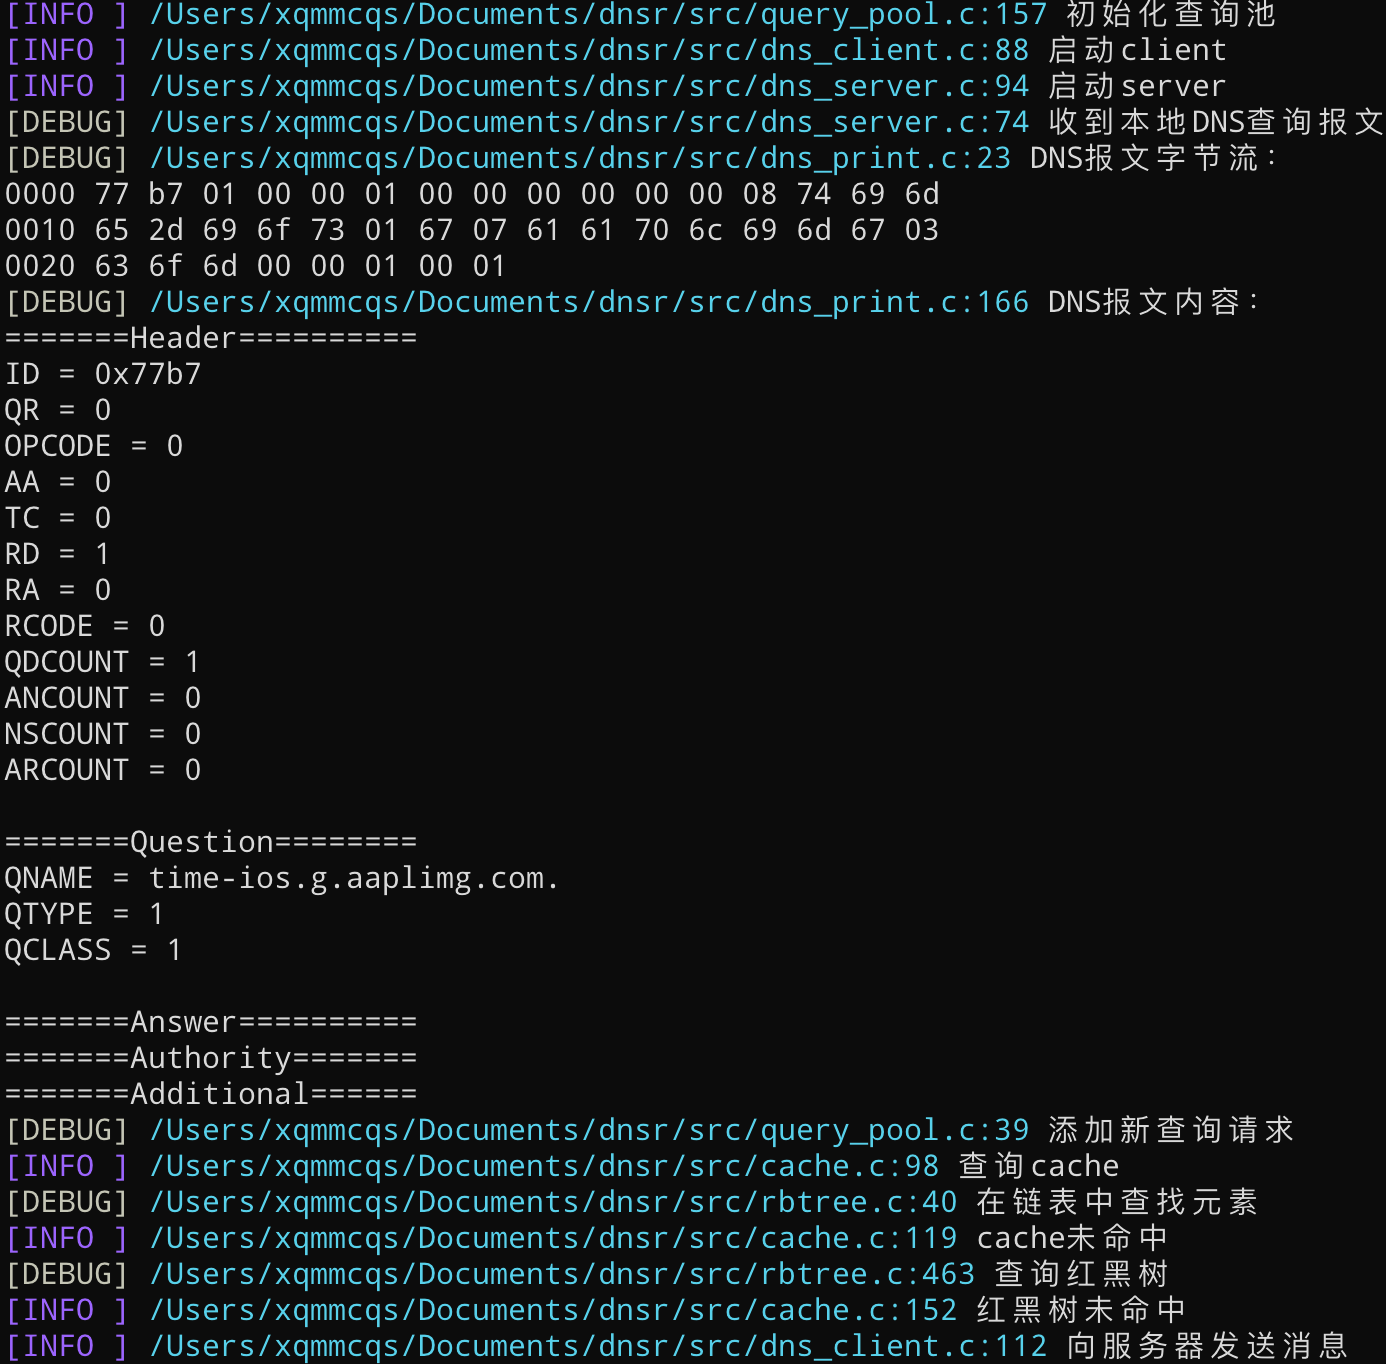
\includegraphics[width=\linewidth]{./Images/log.png}
    \caption{调试信息输出效果\label{fig:log}}

\end{figure}

\section{用户指南}

\subsection{安装依赖}

所需环境:\href{https://github.com/libuv/libuv}{libuv}和\href{https://cmake.org/download/}{CMake}。

Linux下安装libuv:

\begin{code}
\begin{minted}{shell}
apt install libuv1-dev -y
\end{minted}
\end{code}

macOS下安装libuv,首先从GitHub下载源程序,通过以下方式编译:

\begin{code}
\begin{minted}{shell}
sh autogen.sh
./configure
make
make check
make install
\end{minted}
\end{code}

\subsection{编译项目}

libuv安装完成后,需要将\mintinline{text}{CMakeLists.txt}中\mintinline{text}{link_directories}和\mintinline{text}{include_directories}的值改为libuv的动态链接库和头文件路径。

之后,在项目目录中执行以下命令来编译:

\begin{code}
\begin{minted}{shell}
mkdir build
cd build
cmake ..
make
\end{minted}
\end{code}

编译完成后,运行:

\begin{code}
\begin{minted}{shell}
./main
\end{minted}
\end{code}

程序运行参数参考\ref{para}节的说明,例如:

\begin{code}
\begin{minted}{shell}
./main --log_path ./log.txt --remote_host 114.114.114.114
\end{minted}
\end{code}

\subsection{配置DNS服务器}

对于Linux系统,执行如下指令:

\begin{code}
\begin{minted}{shell}
echo 'nameserver 127.0.0.1' >> /etc/resolv.conf
\end{minted}
\end{code}

对于macOS系统,在设置中,进入网络设置,如\figref{fig:settings1},点击“高级...”。之后按照\figref{fig:settings2}中的提示操作,完成后点击\figref{fig:settings1}右下角的“应用”。

\begin{figure}[htbp]

    \centering
    
    \subfigure[网络设置页面\label{fig:settings1}]{
        \begin{minipage}[t]{0.45\linewidth}
            \centering
            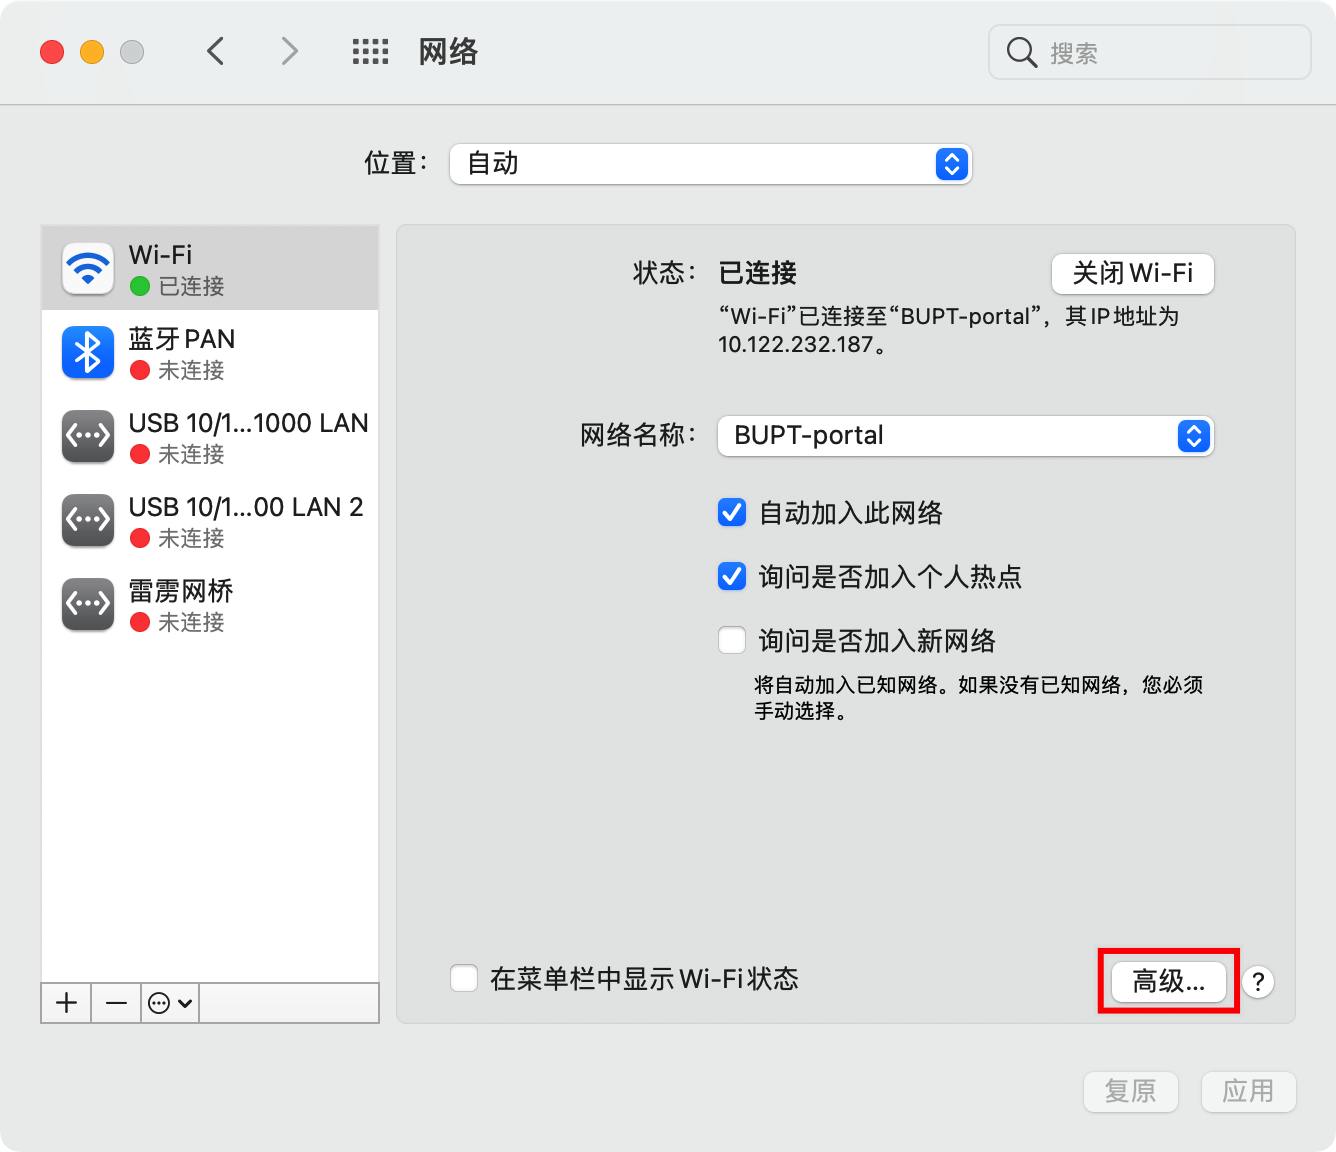
\includegraphics[width=\linewidth]{./Images/settings1.png}
        \end{minipage}
    }
    \subfigure[高级设置\label{fig:settings2}]{
        \begin{minipage}[t]{0.45\linewidth}
            \centering
            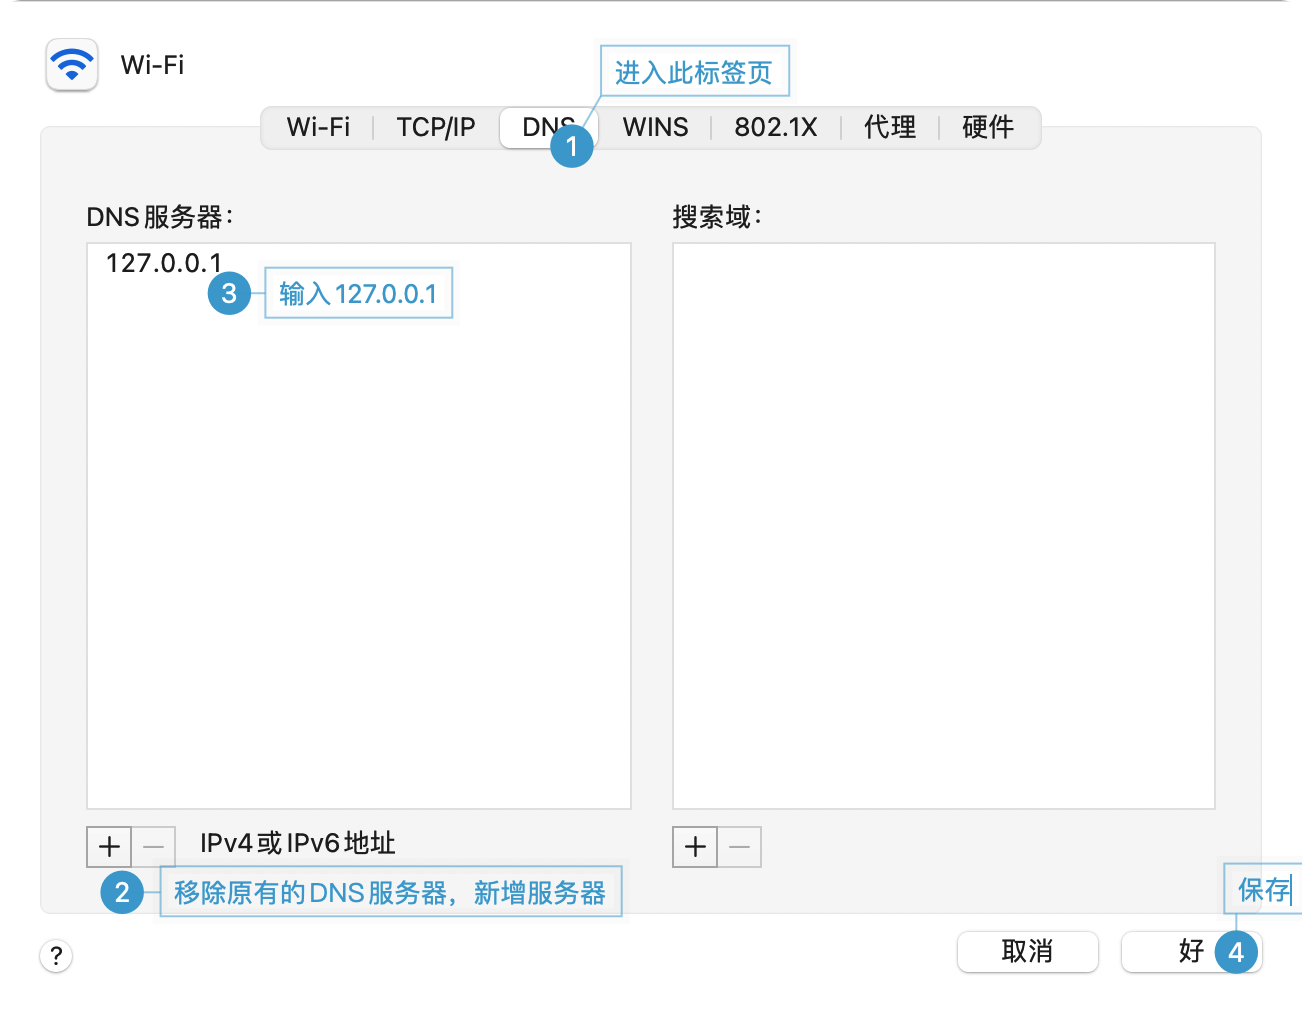
\includegraphics[width=\linewidth]{./Images/settings2.png}
        \end{minipage}
    }
    \caption{网络设置}

\end{figure}

\subsection{抓包与分析}

对于Linux系统,首先使用\mintinline{shell}{ifconfig}查看需要监听的网卡,例如选择\mintinline{text}{eth0}网卡,使用\mintinline{shell}{tcpdump}指令监听UDP端口53,进行抓包:

\begin{code}
\begin{minted}{shell}
tcpdump -i eth0 udp port 53 -vv
\end{minted}
\end{code}

产生的输出如下:

\begin{code}
\begin{minted}{text}
tcpdump: listening on eth0, link-type EN10MB (Ethernet), capture size 262144 bytes
22:05:01.549890 IP (tos 0x0, ttl 64, id 35938, offset 0, flags [DF], proto UDP (17), length 58)
    km-ubuntu.40868 > 222.172.200.68.domain: [bad udp cksum 0x680e -> 0x6b26!] 21821+ A? ourtale.love. (30)
22:05:01.550179 IP (tos 0x0, ttl 64, id 35939, offset 0, flags [DF], proto UDP (17), length 58)
    km-ubuntu.57546 > 222.172.200.68.domain: [bad udp cksum 0x680e -> 0x7e71!] 177+ AAAA? ourtale.love. (30)
22:05:01.551235 IP (tos 0x0, ttl 64, id 35940, offset 0, flags [DF], proto UDP (17), length 73)
...
\end{minted}
\end{code}

或者使用Wireshark软件,选择网卡后,在筛选栏中输入\mintinline{text}{dns},过滤出DNS报文,如\figref{fig:wireshark1}所示。如果想要抓取本地进程和DNS服务端通信的报文,选择网卡Loopback即可,如\figref{fig:wireshark2}。

\begin{figure}[htbp]

    \centering
    
    \subfigure[Wireshark抓取DNS客户端和远程服务器通信的报文\label{fig:wireshark1}]{
        \begin{minipage}[t]{\linewidth}
            \centering
            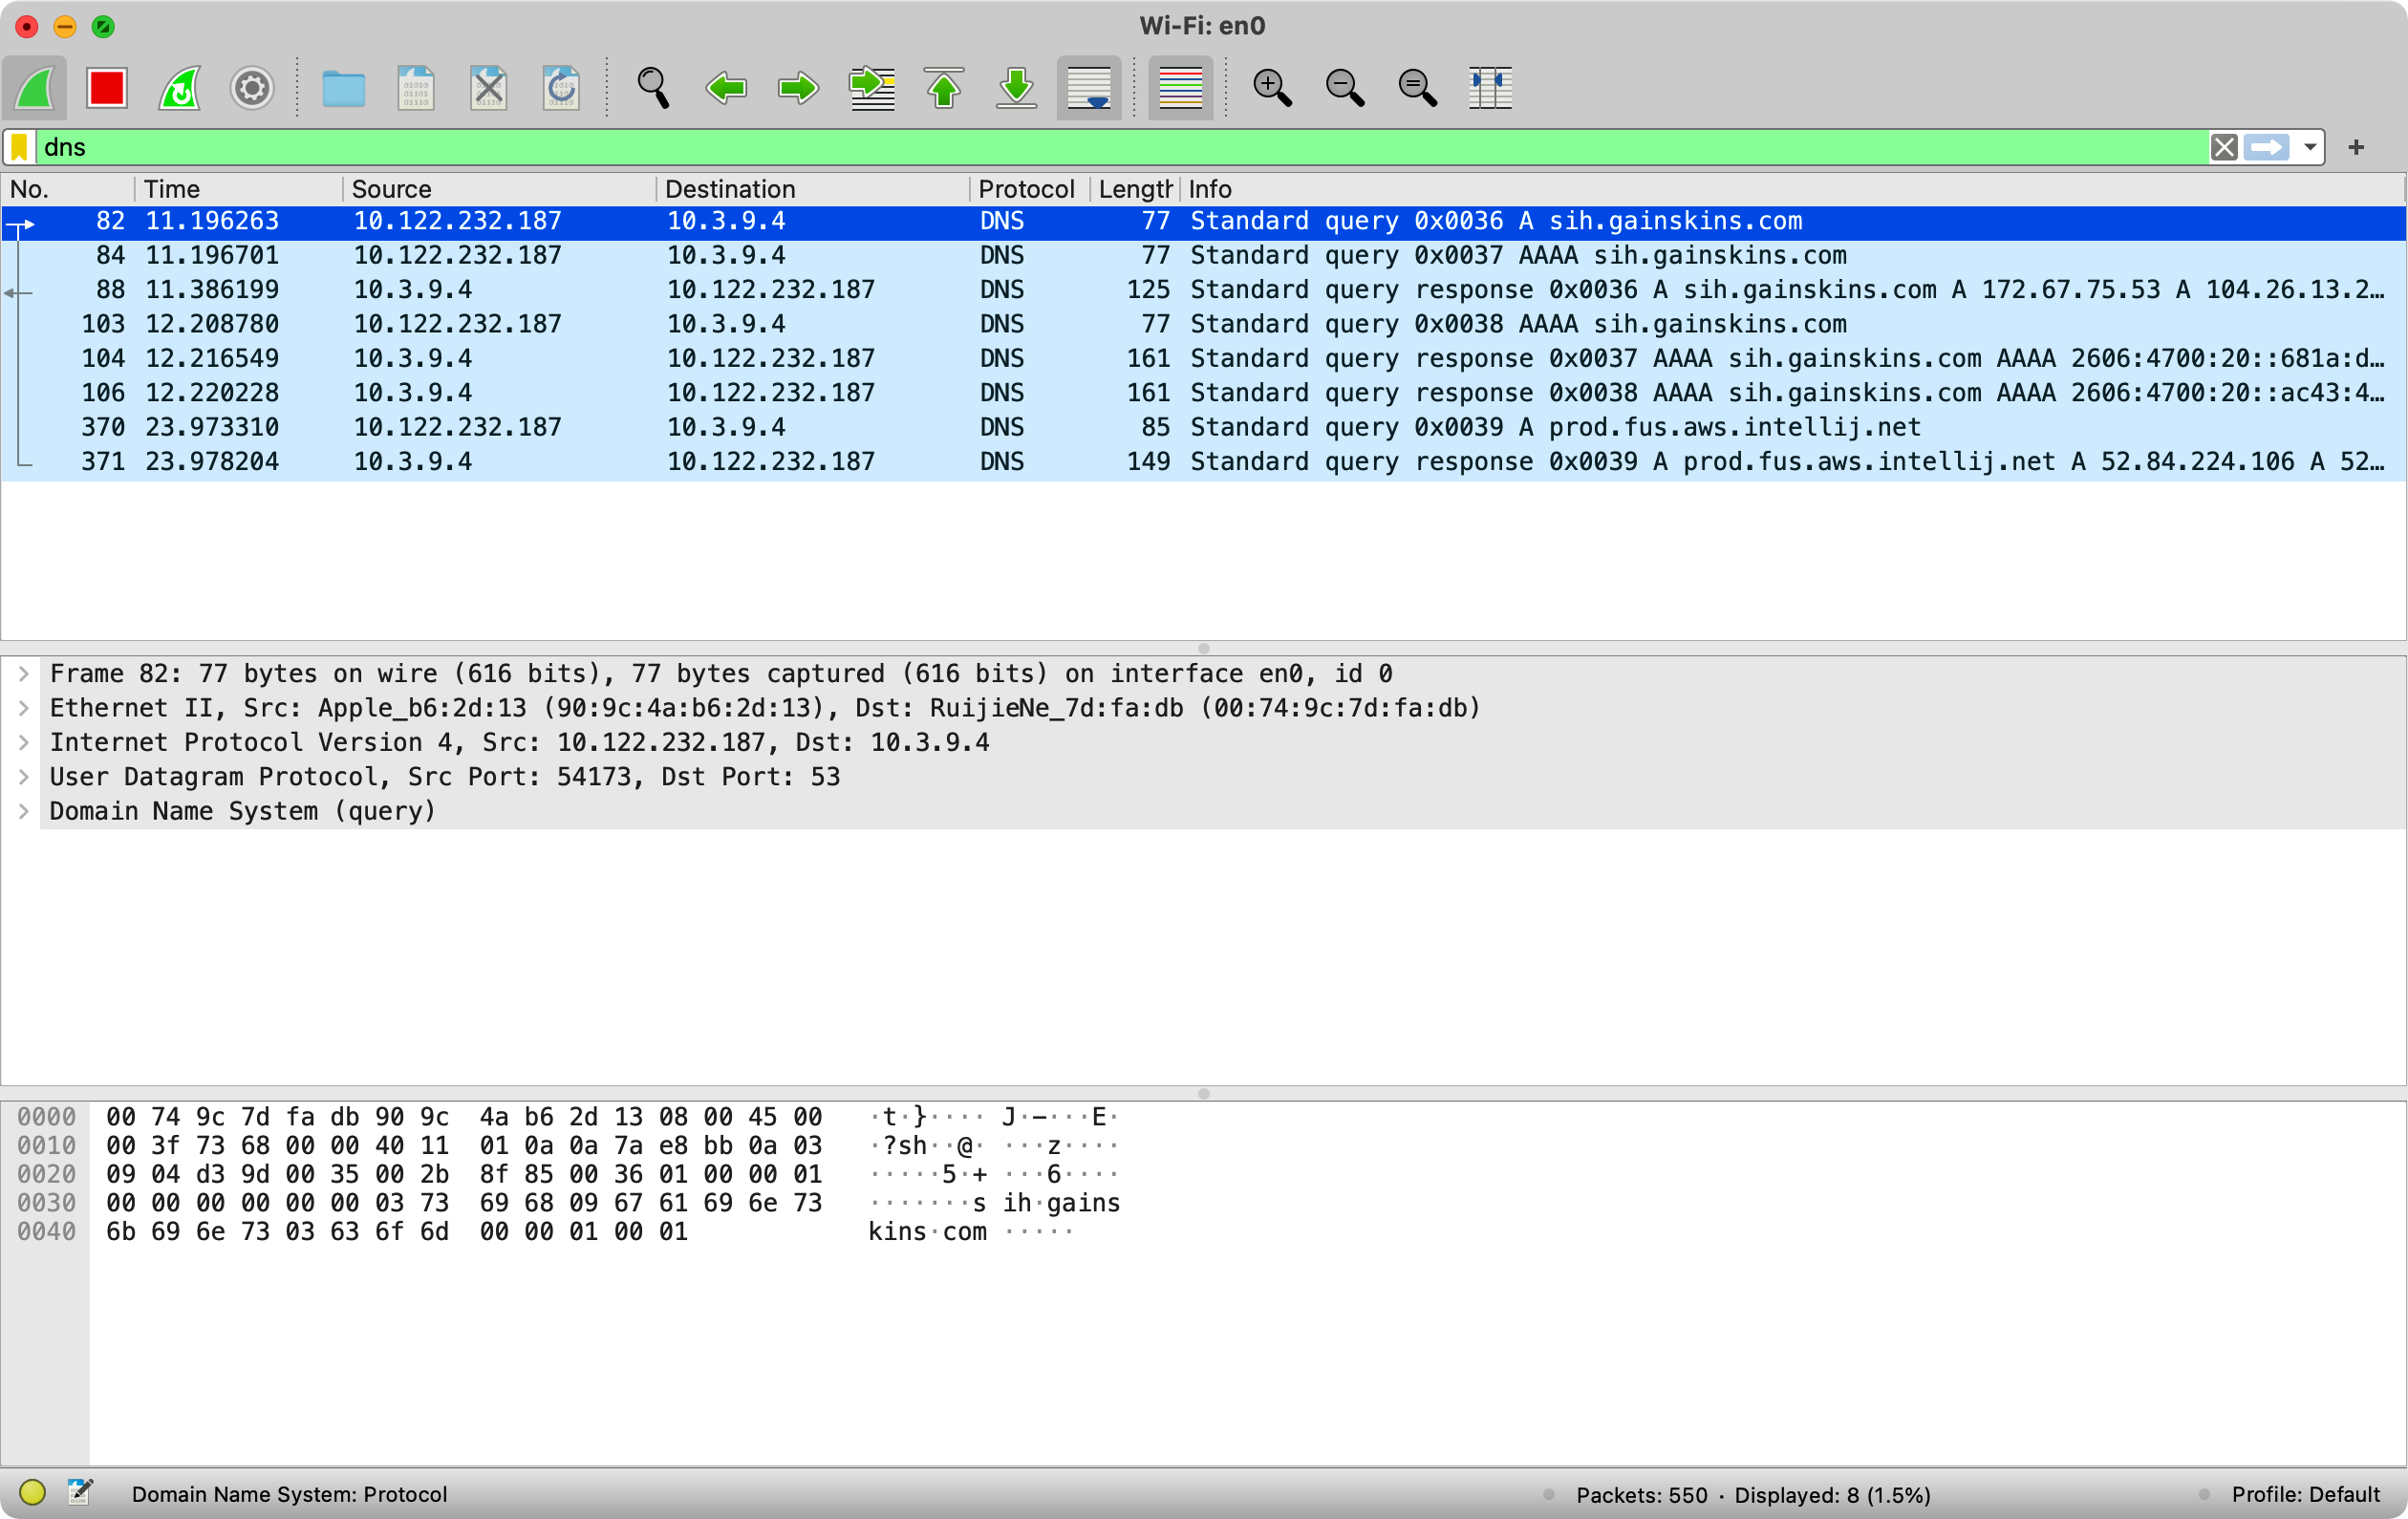
\includegraphics[width=\linewidth]{./Images/wireshark1.png}
        \end{minipage}
    }

    \subfigure[Wireshark抓取本地进程和DNS服务端通信的报文\label{fig:wireshark2}]{
        \begin{minipage}[t]{\linewidth}
            \centering
            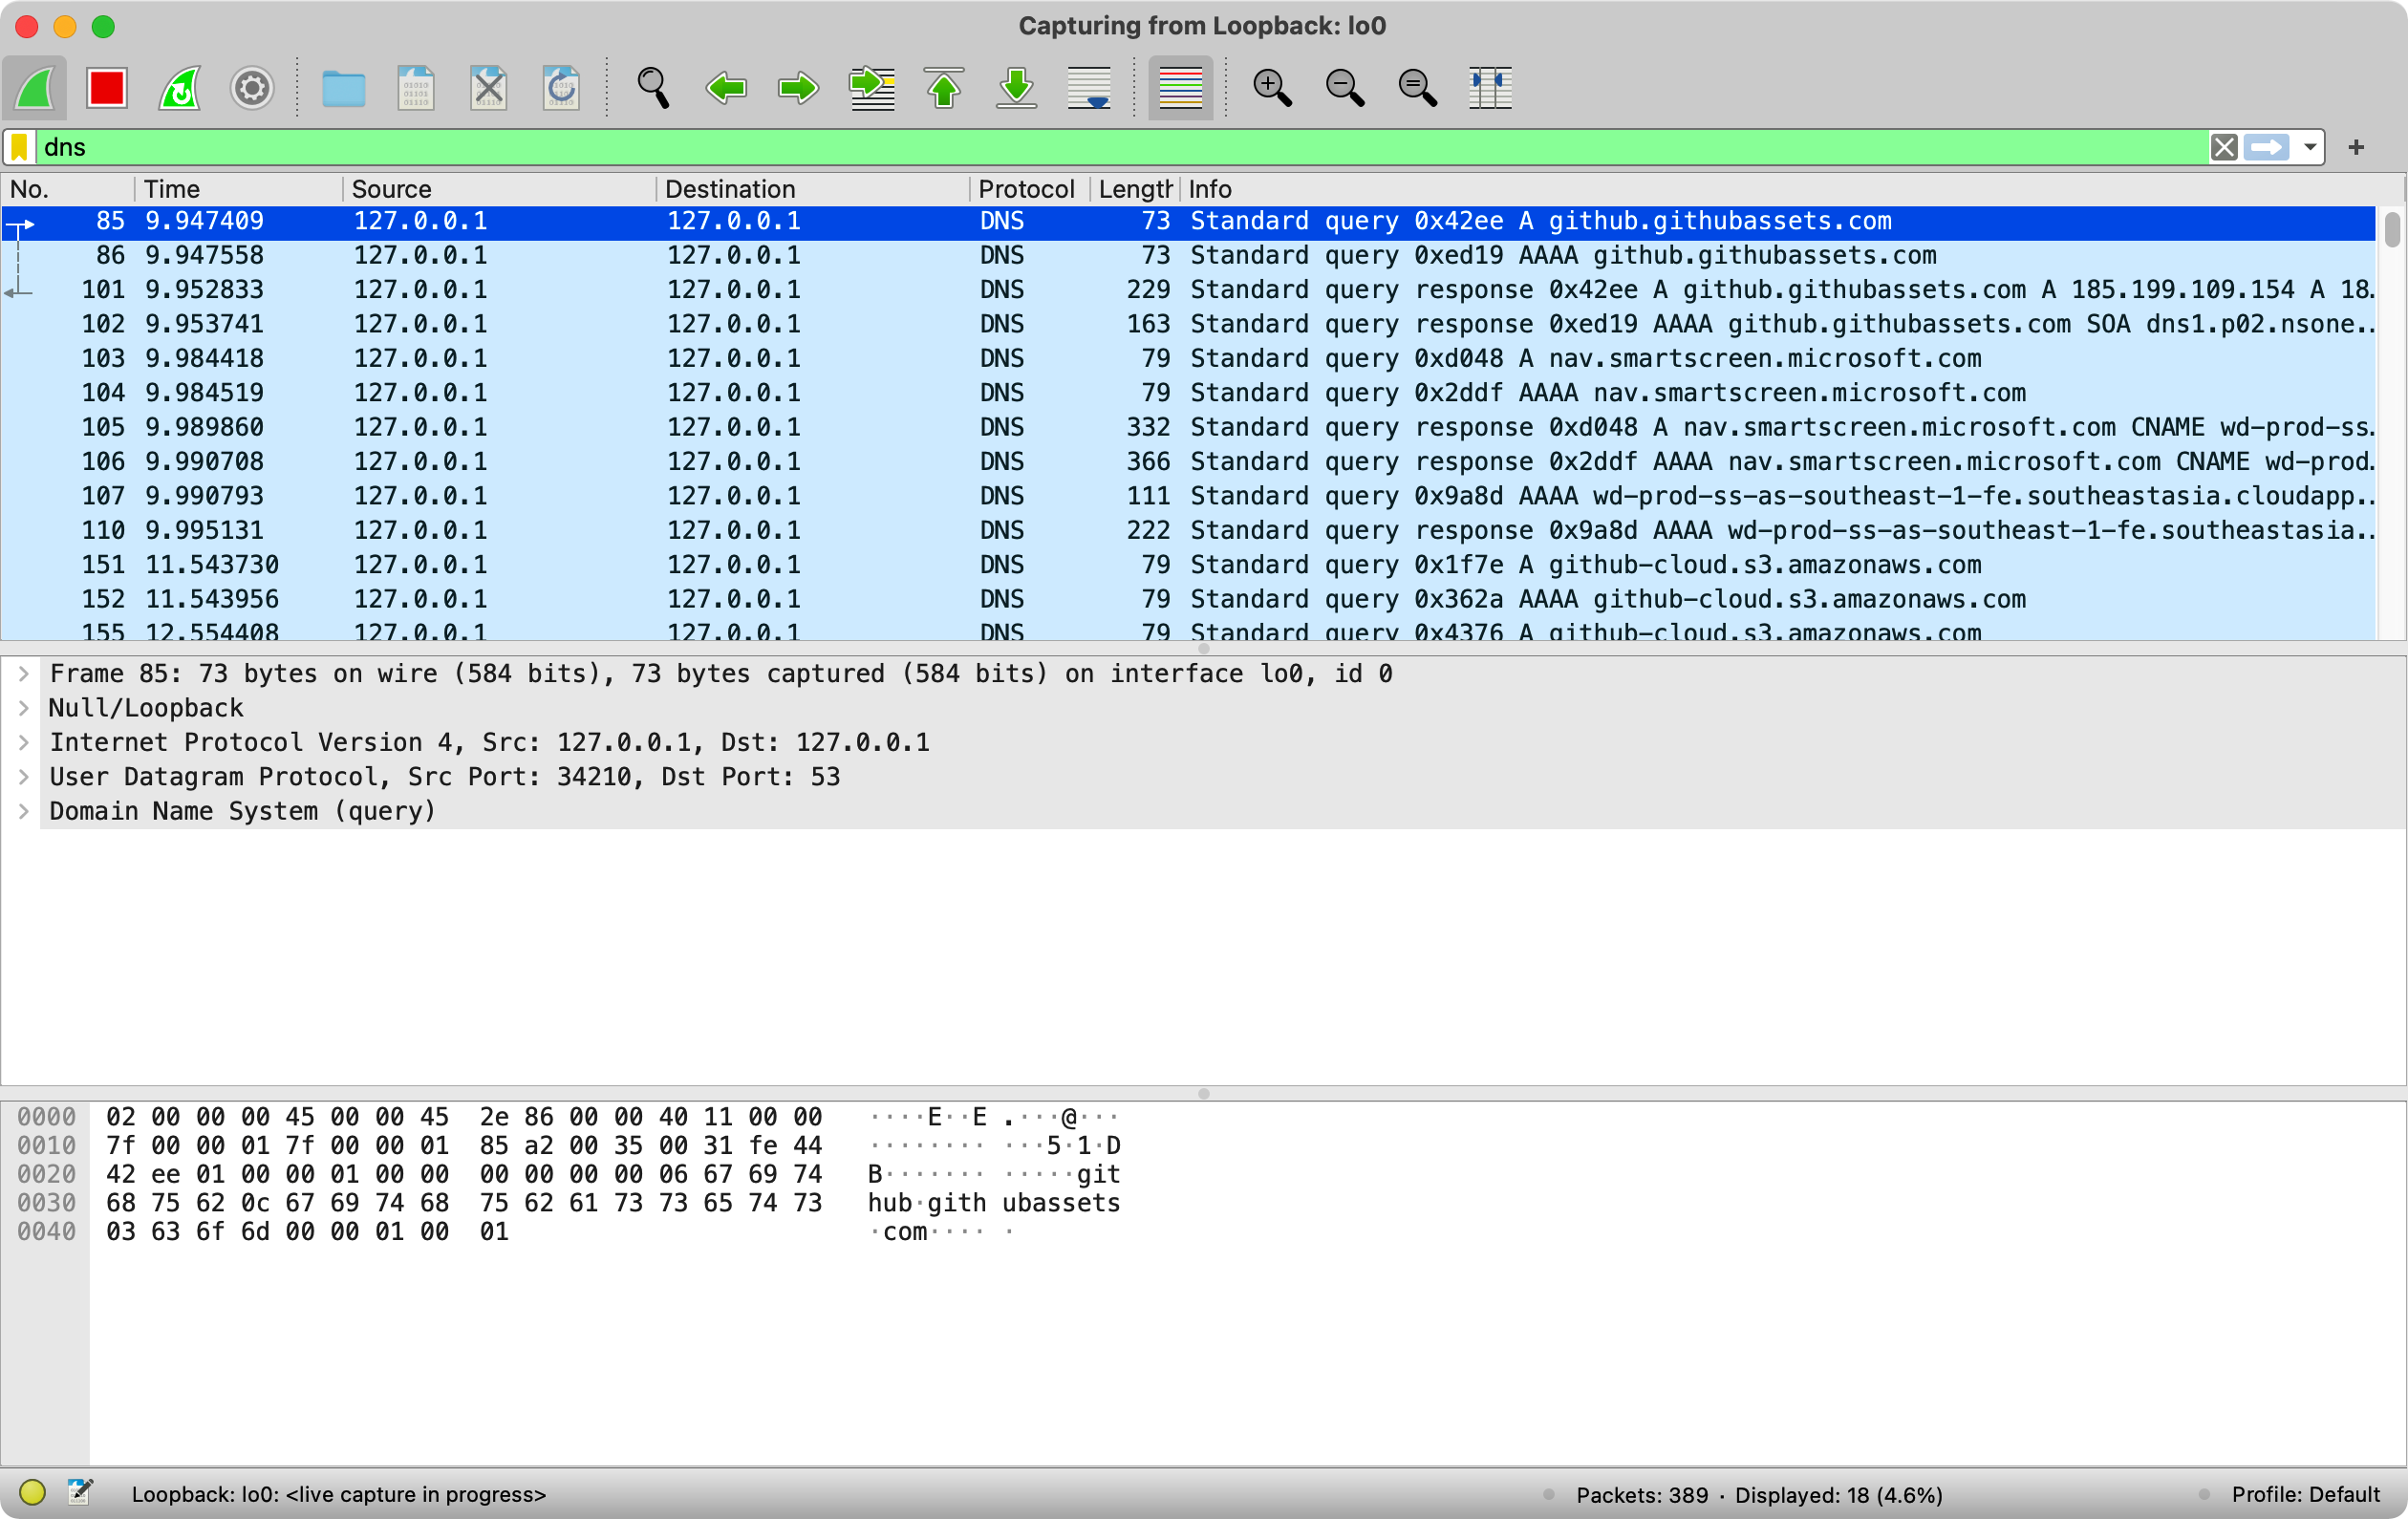
\includegraphics[width=\linewidth]{./Images/wireshark2.png}
        \end{minipage}
    }
    \caption{Wireshark抓包}

\end{figure}

\section{测试结果}

\subsection{基础功能测试}

三个基本功能的测试结果如\figref{fig:test}。对照表采用\ref{iptable}节中的例子。

\begin{figure}[htbp]

    \centering
    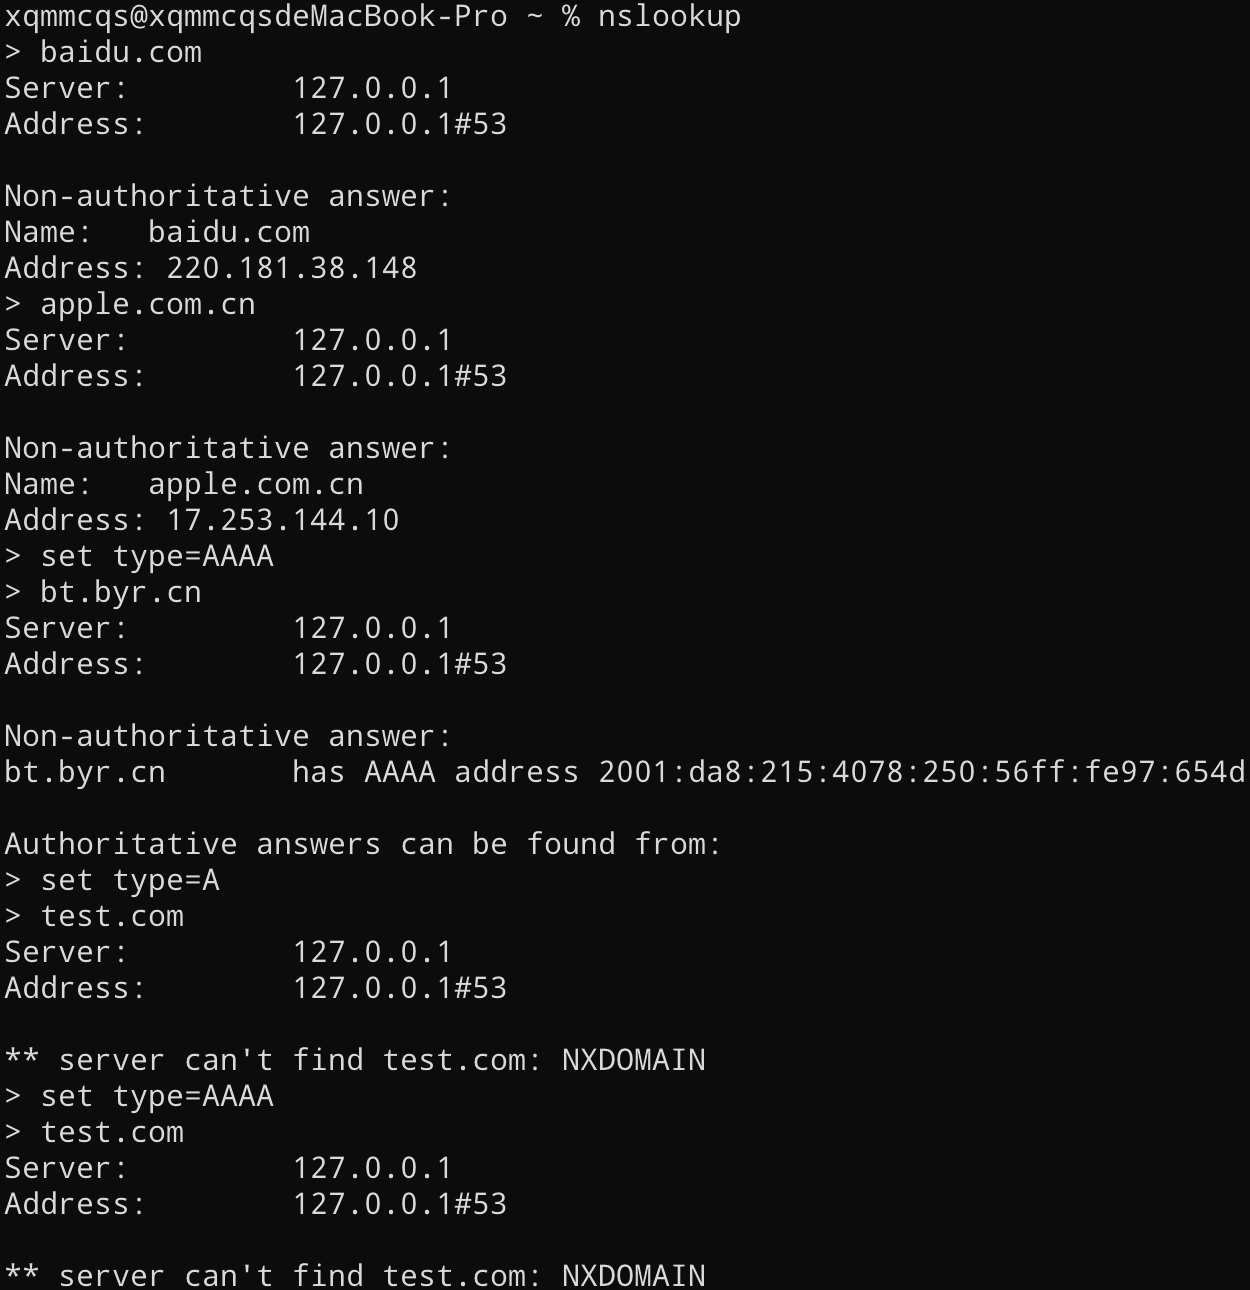
\includegraphics[width=0.7\linewidth]{./Images/test.png}
    \caption{基本功能测试结果\label{fig:test}}

\end{figure}

首先测试了对照表中的域名\mintinline{text}{baidu.com},得到预设的IP,之后测试不在对照表中的域名\mintinline{text}{apple.com.cn},得到正确的IP。

此外,测试了在对照表中的IPv6域名\mintinline{text}{bt.byr.cn},得到预设的IP。最后分别以A类型和AAAA类型测试对照表中设为拦截的域名\mintinline{text}{test.com},会返回查询不到IP的结果。

再次查询\mintinline{text}{apple.com.cn}得到相同的结果,查看报文可知此域名的TTL是10分钟。

经过10分钟,再次查询\mintinline{text}{apple.com.cn},得到相同的结果,查看日志可知,中继服务器删除了红黑树中过期的节点,并且重新向服务器发送查询,如\figref{fig:resend}。

\begin{figure}[htbp]

    \centering
    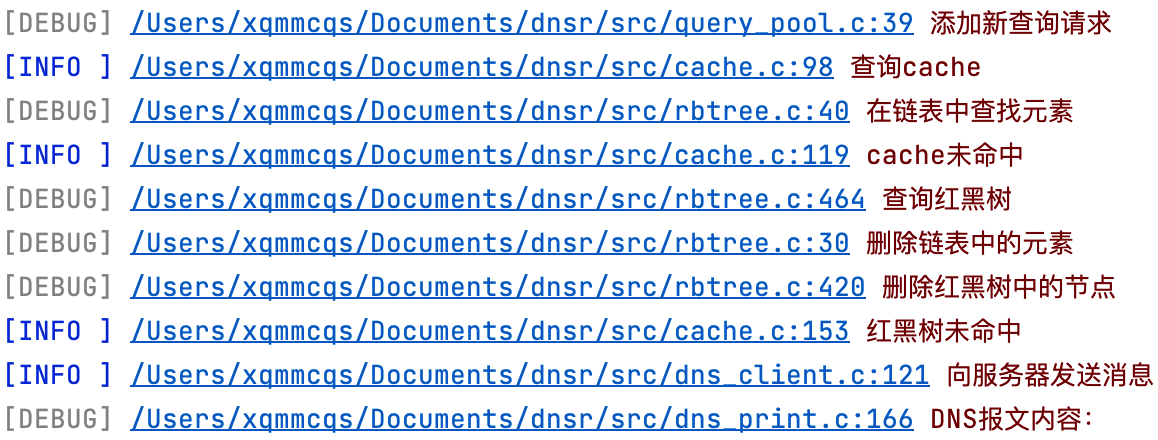
\includegraphics[width=0.7\linewidth]{./Images/resend.png}
    \caption{超时后重新查询的日志\label{fig:resend}}

\end{figure}

\subsection{手动构造报文测试}

通过\mintinline{text}{dnspython}包测试功能,首先执行以下指令安装包:

\begin{code}
\begin{minted}{shell}
pip install dnspython
\end{minted}
\end{code}

手动构造报文:

\begin{code}
\begin{minted}{Python}
from dns import message, query
q1 = message.from_text("id 3000\nopcode QUERY\nrcode NOERROR\nflags RD\n;QUESTION\nbaidu.com. IN A\n;ANSWER\n;AUTHORITY\n;ADDITIONAL")
r = query.udp(a, "127.0.0.1")
print(r.to_text())
\end{minted}
\end{code}

上述代码构造了一个A类型\mintinline{text}{baidu.com}的DNS查询报文,并且向DNS中继服务器发出查询请求,运行结果如下:

\begin{code}
\begin{minted}{text}
id 3000
opcode QUERY
rcode NOERROR
flags QR RD RA
;QUESTION
baidu.com. IN A
;ANSWER
baidu.com. 4294967295 IN A 220.181.38.148
;AUTHORITY
;ADDITIONAL
\end{minted}
\end{code}

我们用这个方法测试了同时发送多个相同编号DNS报文的情况,DNS中继服务器对于每个报文重新编号并且正确地发送了回复。

\subsection{稳定性测试}

运行中继服务器5个小时,期间正常浏览网页、观看视频,服务器没有出现异常。

\section{实验总结}

\subsection{调试中遇到的问题和解决方案}

最初我们期望采用windows和linux系统原生socket接口实现socket编程,我们研究了阻塞式I/O以及常见的跨平台实现。之后我们找到了实现更简单、具有事件驱动和异步I/O功能的libuv库,于是决定采用libuv进行socket编程。

采用libuv实现多线程时,我们遇到了难以调试的内存泄漏和重复释放问题,在参考其他项目的实现之后,我们决定仅采用单线程+事件驱动的形式实现高并发,实测效果与多线程的方式差距不大。

此外,我们的红黑树实现参考了\href{https://zh.wikipedia.org/wiki/%E7%BA%A2%E9%BB%91%E6%A0%91}{维基百科-红黑树}中的实现,但是维基百科中的代码有一些漏洞,比如右旋函数没有判断当前节点是否为根,\mintinline{C}{delete_case}函数中正确的代码被注释掉,这些错误可能导致红黑树中出现二元或者三元环。我们一一修复了这些问题,保证红黑树的正确性。

最后,我们参考常见的实现方法,完成了多个等级的调试信息输出,期间遇到了带有颜色的调试信息无法写入到文件的问题,因此我们需要判断当前输出的文件是否是\mintinline{C}{stderr},再输出颜色信息。

\subsection{工作总结}

本次实验中我们实现了一个功能比较全面的DNS中继服务器,在实用性和效率方面进行了许多改进,使其具有部署到应用环境的价值。

在实验的开始,我们详细研究了DNS协议的内容,阅读RFC 1034和1035文档的重要部分,并且参考一些博客,对报文数据结构的基本格式进行设计。在此期间我们的信息检索能力和英文文献阅读能力均得到了提升。最后,我们通过手动构造报文进行测试,将报文解析结果和Wireshark解析结果进行比对。

在掌握DNS协议的基础知识之后,我们对跨平台socket和高并发的实现进行了研究,最终采用libuv作为解决方案。通过学习libuv的文档和一些示例,我们实现了基础的报文转发功能,并且在高并发的环境下进行了初步的压力测试。

此后,针对高并发查询和重新编号的需求,我们实现了查询池和序号池,在不考虑缓存需求的情况下对这些部分进行了测试。测试结果显示直接中继能够正常运行。

针对缓存的需求,我们学习红黑树和LRU的相关知识,实现了高速缓存+红黑树的两层缓存结构,对于这一个模块进行了单独测试,最后将其整合进主题模块。

最后,我们实现了调试信息模块和命令行参数解析模块,并且参考\href{https://zh-google-styleguide.readthedocs.io/en/latest/google-cpp-styleguide/contents/}{Google开源项目风格指南}和一些其他开源项目,重新格式化了代码,添加了注释,更改了项目的目录结构,完成了文档的撰写工作。

在本次实验中我们主要有如下几个收获:

\begin{itemize}
    \item 了解DNS协议有关知识,掌握DNS协议运作的原理,以及DNS报文的结构。
    \item 掌握跨平台的socket编程技术。
    \item 了解常见的高并发解决方案,理解多线程编程和事件驱动编程的方法。
    \item 学习C语言项目的编码规范,掌握C语言工程的开发和测试方式,了解完整C语言项目的流程,增强C语言编程能力。
    \item 增强英文文档和文献阅读能力和信息检索能力。
\end{itemize}

\appendix

\section{交互式API文档}

由\href{https://www.doxygen.org/index.html}{Doxygen}生成的\href{run:./APIdoc/index.html}{交互式文档}。

\end{document}